% \part*{Introduccion}

% \section*{Convocatoria ordinaria}

% \begin{itemize}
% 	\item P1 - Bloque 1 (14 Nov)
% 	\item P2 - Bloque 2 (20 Dic)
% \end{itemize}

% Requisitos para aprobar por parciales:
% \begin{itemize}
% 	\item P1 \(\geq 3.5\)
% 	\item P2 \(\geq 3.5\)
% 	\item \((P1+P2)/2 \geq 5\)
% \end{itemize}

% \subsection*{Aprobar en el examen de enero}
% \begin{itemize}
% 	\item E1 - Bloque 1 (16 enero)
% 	\item E2 - Bloque 2 (18 enero)
% \end{itemize}
% Se pueden guardar los parciales P1 y P2, que pasan a ser E1 y E2 si no se entrega la prueba correspondiente.

% ...

% \subsection*{Funcionamiento examenes}
% \begin{itemize}
% 	\item Duracion: 90 minutos
% 	\item Teoricos (\(20-30\%\)) y practicos
% 	\item Examenes de enero (E1 y E2) y junio (J1 y J2) \begin{itemize}
% 		      \item 3 horas para hacer las dos pruebas
% 		      \item Se puede entregar una o las dos pruebas. Si no se entrega una se queda la anterior.
% 	      \end{itemize}
% 	\item Aprobando parciales se puede ir a la convocatoria de enero para subir nota (no baja).
% \end{itemize}

% \section*{Bibliografia}
% Apuntes y Problemas de Logica Matematica, Alessandra Gallinari.



\section*{Terminología matemática}

\begin{itemize}
	\item Enunciados:
	      \begin{itemize}
		      \item Teorema
		      \item Proposicion - resultado de un enunciado que propone algo (menor entidad que un teorema)
		      \item Lema - resultado cuya funcion es servir como herramienta auxiliar para probar otra cosa
		      \item Corolario - resultados que se obtienen como consecuencia de demostrar un teorema
		      \item Observacion - puntualizacion verdadera y suficientemente clara como para no necesitar demostracion
		      \item Conjeturas - resultado que se cree que es cierto pero no hay una demostración
	      \end{itemize}
\end{itemize}


Ejemplos:
\begin{theorem}[Ultimo teorema de Fermat]
	Sea \(n \geq  3 \) un numero natural. La ecuacion
	\[
		x^{n } + y^{n} = z^{n}
	\]
	no tiene soluciones (salvo las triviales) en los numeros enteros.
\end{theorem}
\begin{itemize}
	\item Fermat lo enuncia en 1637.
	\item Es una conjetura hasta que Andrew Wiles lo demuestra en 1995.
\end{itemize}
\begin{conjetura}[de Goldbach]
	Sea \(n>2 \) un numero natural par. Entonces \(n \) es suma de dos numeros primos.
\end{conjetura}

\subsection*{Demostracion directa}
\noindent Ejemplos:
\begin{proposition}
	Sea \(n \) un numero natural impar. Entonces la division entera de \( n^{2} \) entre \(8 \) tiene resto \(1\).
\end{proposition}
\begin{proof}
	Como \(n \) es impar, se puede expresar como \(n = 2m + 1 \) con \(m \in  \N \). Asimismo, tenemos que
	\[
		n^{2} = (2m+1)^{2} = 4m^{2} + 4m + 1 \Rightarrow n^{2} = 4m(m + 1) + 1
	\]
	Luego \(m(m+1)\) es un numero par \(\implies \) \(m(m+1 ) = 2 \ell \) con \(\ell \in  \N \).
	\[
		n^{2} = 4 \cdot 2\ell + 1 = 8\ell + 1 \Rightarrow \text{ El resto de \(n^{2}\) entre 8 es 1.}
	\]

\end{proof}

\begin{theorem}[de Pitagoras]
	Sean \(a \) la longitud de la hipotenusa de un triangulo rectangulo y \(b \) y \(c \) las longitudes de sus dos catetos. Entonces se cumple la igualdad
	\[
		a^{2} = b^{2}+c^{2}
	\]
\end{theorem}
\begin{proof}
	Se puede demostrar de forma geométrica:
	\begin{figure}[H]
		\centering
		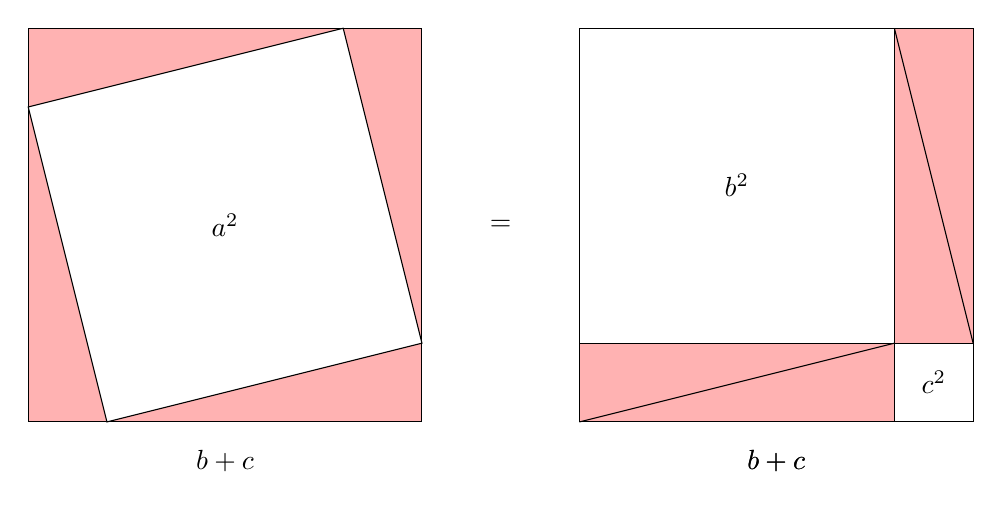
\begin{tikzpicture}

			% Left diagram
			\draw[fill=red!30] (0,0) rectangle (5,5);
			\draw[fill=white] (1,0) -- (5,1) -- (4,5) -- (0,4) -- cycle;

			\node at (2.5,2.5) {$a^2$};
			\node at (2.5,-0.5) {$b+c$};

			% Right diagram
			\begin{scope}[xshift=7cm]
				\draw[fill=red!30] (0,0) rectangle (5,5);
				\draw[fill=white] (0,1) -- (4,1) -- (4,5) -- (0,5) -- cycle;
				\draw[fill=white] (4,0) -- (5,0) -- (5,1) -- (4,1) -- cycle;
				\draw (0,0) -- (4,1);
				\draw (4,5) -- (5,1);

				\node at (2,3) {$b^2$};
				\node at (4.5,0.5) {$c^2$};
				\node at (2.5,-0.5) {$b+c$};

				% Labels
				\node at (2.5,-0.5) {$b+c$};
			\end{scope}

			% Equality sign
			\node at (6,2.5) {$=$};

		\end{tikzpicture}
		\caption{Demostracion del teorema de Pitagoras}
		\label{fig:pitagoras}
	\end{figure}
\end{proof}

\subsection*{Reduccion al absurdo}
Ejemplos:
\begin{theorem}
	\(\sqrt{2} \) es un numero irracional.
\end{theorem}
\begin{proof}
	Lo demostraremos por reduccion al absurdo.

	Supongamos que \(\sqrt{2} \) es un numero racional. Entonces \(\sqrt{2} \) se puede escribir como una fraccion irreducible: \(\sqrt{2 } = \frac{a}{b } \) donde \(a,b \in \Z \) y \(b \neq 0 \). Entonces
	\[
		b\sqrt{2} = a \Rightarrow b^{2}2 = a^{2} \Rightarrow a^{2} \text{ es par} \Rightarrow a \text{ es par} \implies a = 2c
	\]
	Sustituyendo
	\[
		b^{2}2 = (2c)^{2} = 4c^{2} \Rightarrow b^{2} = 2c^{2} \Rightarrow b^{2 } \text{ es par } \Rightarrow \boxed{\text{b es par} }
	\]
	Hay una contradiccion porque \(a \) y \(b \) no tenian factores en comun.

	Luego lo supuesto tiene que ser falso y por tanto \(\sqrt{2} \) \underline{no es racional}.
\end{proof}

\part{Conjuntos, relaciones y funciones}
\section{Conjuntos}
\begin{definition}
	Un conjunto es una coleccion de objetos, que se denominan elementos de ese conjunto.

	Si \(A \) es un conjunto y \(b \) es un elemento de \(A \) decimos que \(b \) pertenece a \(A \). \underline{Notacion:} \(b \in A \).

	En caso contrario, decimos que \(b \) no pertenece a \(A \). \underline{Notacion:} \(b \notin A \).
\end{definition}
Una forma de expresar conjuntos es enumerar sus elementos:
\begin{example}
	\(A = \set{1,3,5,7}\)
\end{example}

\begin{definition}[Subconjunto]
	Sean \(A \) y \(B \) dos conjuntos. Se dice que \(A \) es un subconjunto de \(B \) si todo elemento de \(A \) es tambien elemento de \(B \).

	Tambien se dice que \(A \) esta contenido en \(B \). \underline{Notacion:} \(A \subseteq B \).

	En caso contrario diremos que \(A \) no esta contenido en B.

	\underline{Notacion:} \( A \not\subseteq B\).
\end{definition}

\begin{definition}
	Sean \(A \) y \(B \) dos conjuntos. Decimos que \(A \) y \(B \) son iguales si tienen los mismos elementos. Esto es lo mismo que decir que \(A \subseteq B \) y \(B \subseteq A \).

	\underline{Notacion:} \(A = B \).

	En caso contrario, diremos que \(A \) y \(B \) son distintos.

	\underline{Notacion:} \(A \neq B \).
\end{definition}

\begin{remark}
	En un conjunto no se tienen en cuenta elementos repetidos.

	Tampoco se tiene en cuenta el orden.
\end{remark}
\begin{definition}[Contenido estricto]
	Decimos que A esta estrictamente contenido en \(B \) si \(A \subseteq B \) y \(A \neq  B \).
	Notacion: \(A \subset B \).
\end{definition}

La segunda forma de expresar conjuntos consiste en indicar una propiedad.

\begin{example}
	\[
		A = \set{x \mid x \text{ es un numero primo menor que 15} }
	\]
	\[
		A = \set{2,3,5,7,11,13}
	\]
	\[
		B = \set{x \mid x \text{ es un numero primo mayor que 15} }
	\]
	\[
		B = \set{17,19,23,29,31,37,41,43,\ldots}
	\]
\end{example}

\begin{definition}[Conjuntos numericos, informal]
	~
	\begin{itemize}
		\item Numeros naturales: \\
		      \(\N \coloneqq \set{1,2,3,4,5,\ldots} \). No tiene solucion \(2 - x = 5 \).
		\item Numeros enteros: \\
		      \(\Z \coloneqq \set{\ldots,-2,-1,0,1,2,\ldots }\). No tiene solucion \(2x = 5 \).
		\item Numeros racionales: \\
		      \(\Q \coloneqq \left\{\frac{a}{b} \mid a,b \in \Z, b \neq 0 \right\}\). Tienen expresion decimal periodica. No tiene solucion \(x^{2} = 2 \).
		\item Numeros reales: \\
		      \(\R \). Tienen expresion decimal arbitraria, periodica o no periodica. No tiene solucion \(x^{2} = -1 \).
		\item Numeros complejos: \\
		      \(i \coloneqq \sqrt{-1} \) la unidad imaginaria.

		      \(\C \coloneqq \set{a + bi \mid a,b \in \R}\)
	\end{itemize}
\end{definition}

\begin{definition}
	Se define el conjunto vacio como un conjunto sin elementos.

	\underline{Notacion:} \(\varnothing\)
\end{definition}

\begin{proposition}
	Sea \(A \) un conjunto cualquiera. Se cumple que \(\varnothing \subseteq  A \).
\end{proposition}
\begin{proof}
	Lo demostraremos por reduccion al absurdo.

	Supongamos que \(\varnothing \not\subseteq A \). Entonces, existe un elemento \(x \) tal que \(x \in \varnothing\) y \(x \notin A \).

	Esto es una contradiccion, ya que el conjunto \(\varnothing \) no tiene elementos.

	Luego es falso que \(\varnothing \not\subseteq A \) y por tanto \(\varnothing \subseteq A \).
\end{proof}

\begin{definition}[Operaciones con conjuntos]
	Sean \(A \) y \(B \) dos conjuntos. Se definen:
	\begin{itemize}
		\item Interseccion de \(A \) y \(B \): \\
		      \(A \cap B \coloneqq \set{x \mid x \in A \text{ y } x \in B}\)
		\item Union de \(A \) y \(B \): \\
		      \(A \cup B \coloneqq \set{x \mid x \in A \text{ o } x \in B}\)
		\item Diferencia entre \(A \) y \(B \) (o \(A \) menos \(B \)):

		      \(A \setminus B \coloneqq \set{x \mid x \in A \text{ y } x \notin B }\)

	\end{itemize}
\end{definition}

\begin{definition}
	Decimos que un conjunto \(A \) es finito si tiene tantos elementos como un numero natural o bien si no tiene elementos (\(\varnothing\)).

	En caso contrario decimos que \(A \) es infinito.
\end{definition}

\begin{definition}
	Si \(A \) es un conjunto finito, se define el cardinal de \(A \) como su numero de elementos. El cardinal de \(\varnothing \) es 0. Si \(A \) es un conjunto infinito tiene cardinal infinito.

	\underline{Notacion:} \(|A|\)
\end{definition}

\begin{definition}[Partes de un conjunto]
	Sea \(A \) un conjunto. Se define el conjunto de las partes de \(A \) como el conjunto formado por todos los subconjuntos de \(A \). Simbolicamente:
	\[
		\mathcal{\MakeUppercase{P}}(A) = \set{B \mid B \subseteq A }
	\]
\end{definition}
\begin{example}
	Sean \(A = \set{1,2}\), \(B = \set{1,2,3}\), \(C = \set{1,2,3,4}\). Escribir los conjuntos \(\mathcal{\MakeUppercase{P}}(A), \mathcal{\MakeUppercase{P}}(B), \mathcal{\MakeUppercase{P}}(C), \mathcal{\MakeUppercase{P}}(\mathcal{\MakeUppercase{P}}(A))\).
	\begin{itemize}
		\item Subconjuntos de \(A \): \(\set{1}, \set{2}, \set{1,2}, \varnothing\).

		      Luego \(\mathcal{\MakeUppercase{p}}(A) = \set{\varnothing, \set{1}, \set{2},\set{1,2}}\)

		\item Subconjuntos de \(B \): \(\set{1},\set{2},\set{3},\set{1,2}, \set{1,3}, \set{2,3}, \set{1,2,3}, \varnothing\).

		      Luego \(\mathcal{\MakeUppercase{p}}(B) = \set{\varnothing, \set{1}, \set{2}, \set{3}, \set{1,2}, \set{1,3}, \set{2,3}, \set{1,2,3}}\)
	\end{itemize}
\end{example}

\begin{theorem}
	Sea \(A \) un conjunto finito. Entonces se cumple que
	\[
		|\mathcal{\MakeUppercase{p}}(A)| = 2^{|A|}
	\]
\end{theorem}
\begin{proof}
	Considero el conjunto \(A \) formado por \(n \) elementos donde \(n \in \N\).

	Sin perdida de generalidad, supongo que \(A = \set{1,2,3,\ldots,n}\). Para contar subconjuntos de \(A \), planteo el cuestionario \begin{enumerate}
		\item ¿Está 1 en el subconjunto?
		\item ¿Está 2 en el subconjunto?
		\item[n.] ¿Está \(n \) en el subconjunto?
	\end{enumerate}
	Hay el mismo numero de subconjuntos de \(A \) que de respuestas al cuestionario. Como el cuestionario tiene \(n \) preguntas y cada una 2 respuestas posibles, hay \(2^{n } \) respuestas diferentes al cuestionario y, por tanto, \(2^{n } \) subconjuntos de \(A \).

	Falta probarlo para \(A = \varnothing\). Se cumple que \(\varnothing \subseteq \varnothing\) y es el unico posible.

	Luego \(\mathcal{\MakeUppercase{p}}(\varnothing) = \set{\varnothing}\)

	Tenemos que \(|A| = 0 \) y \(|\mathcal{\MakeUppercase{p}}(A)| = 1\). Ademas, \(2^{|A|} = 2^{0} = 1 = |\mathcal{\MakeUppercase{p}}(A)|  \)
\end{proof}
\begin{proof}
	Tambien lo demostraremos por induccion sobre \(n \), el numero de elementos de \(A \).

	El caso \(n = 0 \) esta hecho en la demostracion anterior.

	En el caso base, \(n = 1\), \(A = \set{1 }\) y \(\mathcal{\MakeUppercase{p}}(A) = \set{\varnothing, \set{1}}\). Luego \(|A| = 1 \) y \(|\mathcal{\MakeUppercase{p}}(A)| = 2 = 2^{1} = 2^{|A| } \). Se cumple para \(n = 1 \).

	Hipotesis de induccion: Supongamos que el resultado es cierto para \(n \) (\(A = \set{1,2,3,\ldots,n}\) y \(|\mathcal{\MakeUppercase{p}}(A)| = 2^{n}  \))

	Tengo que demostrar, a partir de esto, la tesis de induccion:

	Si \(B = \set{1,2,3,\ldots,n,n+1}\) entonces \(|\mathcal{\MakeUppercase{p}}(A)| = 2^{n+1} \).

	Hay 2 tipos de subconjuntos de \(B \).
	\begin{description}
		\item[Tipo 1] Los que no tienen a \(n+1 \) como elemento. Por hipotesis de induccion hay \(2^{n } \) subconjuntos de \(B \) de este tipo (son los mismos que los de \(A \)).
		\item[Tipo 2] Los que si tienen a \(n+1 \) como elemento. Cada uno de estos se obtiene añadiendo el elemento \(n+1\) a un subconjunto de \underline{Tipo 1}. Por tanto, hay tantos como habia de Tipo 1: \(2^{n} \).
	\end{description}
	En total, \(B \) tiene:
	\[
		\underbrace{2^{n}}_{\text{Tipo 1}} + \underbrace{2^{n}}_{\text{Tipo 2}} = 2 \cdot 2^{n} = 2^{n+1} = |\mathcal{\MakeUppercase{p}}(B)|
	\]
	Asi, queda demostrada la tesis de induccion.
\end{proof}

\begin{definition}[Par ordenado]
	Dados dos conjuntos \(A \) y \(B \) y dos elementos \(a \in  A\) y \(b \in B \), se define el \underline{par ordenado} formado por \(a \) y \(b \) como la expresion simbolica
	\[
		(a,b)
	\]
	donde \(a \) es el primer elemento del par y \(b \) es el segundo elemento del par.
\end{definition}

\begin{definition}[Producto cartesiano]
	Sean \(A \) y \(B \) dos conjuntos no vacios. Se define el producto cartesiano de \(A \) por \(B \) como el conjunto formado por todos los pares ordenados de la forma \((a,b )\) donde \(a \in A \) y \(b \in B \). Simbolicamente:
	\[
		A \times B \coloneqq \set{(a,b) \mid a \in A, b \in B}
	\]
\end{definition}
\begin{example}
	\(A = \set{1,2,3}\), \(B = \set{2,4}\)
	\[
		A \times B = \set{(1,2), (1,4), (2,2), (2,4), (3,2), (3,4)}
	\]
	\[
		B \times A = \set{(2,1), (2,2), (2,3), (4,1), (4,2), (4,3)}
	\]
	El producto cartesiano no es conmutativo.
\end{example}

\begin{proposition}
	Sean \(A \) y \(B \) dos conjuntos finitos y no vacios. Se cumple que
	\[
		| A \times B | = |A| \cdot |B|
	\]
\end{proposition}
\begin{proof}
	Para formar todos los pares ordenados posibles, tenemos \(|A| \) opciones en la primera coordenada y \(|B| \) en la segunda.

	Por tanto, hay en total \(|A| \cdot |B| \) pares ordenados.

	Así, \(|A \times B| = |A| \cdot |B|\)
\end{proof}

\begin{remark}
	Si \(A \) o \(B \) es infinito \(\Rightarrow \) \(|A \times B| = \infty\)
\end{remark}

\begin{definition}[n-tupla ordenada]
	Sea \(n \in  \N \), \(n \geq  2 \). Sean \(A_1, A_2, \ldots, A_n \) conjuntos y \(a_1 \in  A_1 \), \(a_2 \in A_2 \), \(\ldots \), \(a_n \in A_n \) elementos de sus conjuntos. Se define la n-tupla ordenada formada por esos elementos como la expresion simbolica
	\[
		(a_1, a_2, \ldots, a_n )
	\]
\end{definition}
\begin{definition}
	Sea \(n \in \N \), \(n \geq  2\). Sean \(A_1, A_2, \ldots, A_n \) conjuntos no vacios. Se define el producto cartesiano de esos conjuntos como
	\[
		A_1 \times A_2 \times \dots \times A_n \coloneqq \set{(a_1,a_2,\dots,a_n) \mid a_1 \in A_1, a_2 \in A_2, \ldots, a_n \in A_n}
	\]

\end{definition}

Si hacemos el producto cartesiano de un conjunto no vacio \(A \) por si mismo varias veces, usaremos
\[
	A^{n} \coloneqq A \times A \times \dots A \text{ (n veces)}
\]

\section{Relaciones}

\begin{definition}[Relacion binaria de dos conjuntos]
	Sean \(A \) y \(B \) dos conjuntos no vacios. Una relacion binaria entre \(A \) y \(B \) es un subconjunto \(R \subseteq A \times B \).
\end{definition}

\begin{definition}[Relacion binaria en un conjunto]
	Sea \(A \) un conjunto no vacio. Una relacion binaria en \(A \) es ub subconjunto \(R \subseteq A \times A \).
\end{definition}

Sea \(R \) una relacion entre dos conjuntos \(A \) y \(B \). Si \((a,b) \in R \) decimos que a esta relacionado con b por \(R \) y escribimos: \(a R b\)

\begin{example}
	\(A \times B = {1,2,3} \times {2,4}\).

	Una relacion es \(R_1 = \set{(1,2),(1,4 )}\) o \(R_2 = \set{(1,2), (2,2), (3,4)}\).
	El producto cartesiano \(A \times B \) o \(\varnothing\) tambien son relaciones.
\end{example}

\begin{remark}
	Como \(A \times B \) tiene \(6 \) elementos, puedo encontrar \(2^{6} = 64 \) relaciones distintas (porque \(A \times B \) tiene 64 subconjuntos distintos).
\end{remark}

%% Cuantificadores 

\begin{definition}[Dominio, imagen]
	Sea \(R \) una relacion binaria entre dos conjuntos \(A \) y \(B \). Se definen
	\begin{itemize}
		\item Dominio de \(R \) como
		      \[
			      dom(R) \coloneqq \set{a \in  A \mid \exists b \in B \mid a R b}
		      \]
		\item Imagen o rango de \( R \) como
		      \[
			      im(R) \coloneqq \set{ b \in B \mid \exists a \in  A \mid a R b}
		      \]
	\end{itemize}
\end{definition}

\begin{definition}
	Sea \(R \) una relacion binaria entre dos conjuntos \(A \) y \(B \). Sean \(C \subseteq A \) y \(D \subseteq B \). Se definen:
	\begin{itemize}
		\item Imagen inversa de \(D \) por \(R \) como
		      \[
			      R^{-1}(D) \coloneqq \set{a \in  A \mid \exists  b \in  D \mid a R b}
		      \]
		\item Imagen o imagen directa de \(C \) por \(R \) como
		      \[
			      R(C) \coloneqq \set{b \in B \mid \exists a \in  C \mid aRb}
		      \]
	\end{itemize}
\end{definition}
\begin{remark}
	\[
		dom(R) = R^{-1}(B)
	\]
	\[
		im(R) = R(A)
	\]
\end{remark}

\begin{example}
	Sean \(A = \set{1,3,5 }\), \(B = \set{2,3 }\), \(C = \set{1,3} \subseteq A \), \(D = \set{2} \subseteq B \).
	\begin{itemize}
		\item \(R_1  = \set{(1,2),(3,2), (3,3)}\)
		      \[
			      dom(R_1) = \set{1,3}, \, im(R_1) = \set{2,3}, \,R^{-1}_1(D) = \set{1,3}, \, R_1(C) = \set{2,3}
		      \]
		\item \(R_2 = \set{(1,2), (3,3), (5,2)}\) - Funcion.
		      \[
			      dom(R_2) = A, im(R_2) = B, R^{-1}_2(D) = \set{1,5}, R_2(C) = \set{2,3} =B
		      \]
	\end{itemize}
	En total habia \(2^{6}  \) relaciones entre \(A \) y \(B \).
\end{example}

\begin{example}
	Sean \(A = \set{1,2,4,5}\), \(C = \set{2,5} \subseteq A \).
	\begin{itemize}
		\item \(R_1 = \set{(x,y) \mid x = y }\)
		      \[
			      dom(R_1) = A, im(R_1) = A, R^{-1}_1 (C) = \set{2,5} =C, R_1(C) = \set{2,5} =C
		      \]
		\item \(R_2 = \set{(x,y) \mid x \neq y } = A^{2} \setminus R_1 \)
		      \[
			      dom(R_2) = A, im(R_2) = A, R^{-1}_2 (C) = A, R_2 (C) = A
		      \]
		\item \(R_3 = \set{(x,y) \mid x < y }\)
		      \[
			      dom(R_3) = \set{1,2,4}, im(R_4) = \set{2,4,5}, R^{-1}_3 (C) = \set{1,2,4}, R_3 (C) = \set{4,5}
		      \]
		\item \(R_4 = \set{(x,y) \mid x \leq y } = R_1 \cup R_3\)
		      \[
			      dom(R_4) = A, im(R_4)=A, R^{-1}_4 (C) = A, R_4 (C) = \set{2,4,5}
		      \]
		\item \(R_5 = \set{(x,y) \mid x \text{ es divisor de } y} = \set{(1,1), (1,2), (1,4), (1,5), (2,2), (2,4), (4,4), (5,5)}\)
		      \[
			      dom(R_5) = A, im(R_5) = A, R^{-1}_5(C) = \set{2,4,5}, R_5(C) = \set{2,4,5}
		      \]
		\item \(R_6 = \set{(1,1), (1,4), (2,4 )}\)
		      \[
			      dom(R_6) = \set{1,2}, im(R_6) = \set{1,4}, R^{-1}_6(C)=\varnothing, R_6(C) = \set{4}
		      \]
	\end{itemize}
\end{example}

\begin{definition}
	Sean \(P \) y \(Q\) dos enunciados. La notacion
	\[
		P \Rightarrow Q
	\] se lee ``\(P \) implica \(Q \)''.

	El unico caso en el que es falsa es cuando sucede \(P \) y no sucede \(Q \). Esta situacion supone un contraejemplo a la implicacion.

	La notacion
	\[
		P \iff  Q
	\]
	se lee ``\(P \) si y solo si \(Q \)'' o ``\(P \) es equivalente a \(Q \)'' y quiere decir que \(P \Rightarrow Q \) y \(Q \Rightarrow P \) simultaneamente. Es falsa si sucede una de las dos afirmaciones y no la otra.
\end{definition}

\begin{definition}
	Sean \(A \) un conjunto no vacio y \(R \) una relacion binaria en \(A \). Decimos que \(R \) cumple la propiedad
	\begin{itemize}
		\item Reflexiva si \(\forall x \in  A \;(xRx )\)
		\item Simetrica si \(\forall x,y \in  A \;(xRy \Rightarrow yRx )\)
		\item Antisimetrica si \(\forall  x,y \in A \;(xRy, x \neq y \Rightarrow y \cancel R z)\) \\
		      También se puede formular: \(\forall x,y \in  A \; (xRy, yRx \Rightarrow x = y)\)
		\item Transitiva si \(\forall x,y,z \in A \; (xRy, yRz \Rightarrow xRz)\)
	\end{itemize}
\end{definition}

\begin{definition}
	Sean \(A \) un conjunto no vacio y \(R \) una relacion binaria en \(A \). Decimos que \(R \) es una relacion de
	\begin{itemize}
		\item Equivalencia si cumple las propiedades reflexiva, simetrica y transitiva.
		\item Orden si cumple las propiedades reflexiva, antisimetrica y transitiva.
		\item Orden total si es de orden y ademas \(\forall x,y \in A \; (xRy \text{ o } yRx )\)
	\end{itemize}
\end{definition}

\begin{example}
	Sea \(A = \set{a,b,c,d}\). Para cada una de las siguientes relaciones \(R_i \) en \(A \), estudia si cumplen las propiedades reflexiva, simetrica, antisimetrica y transitiva. Tambien si son de equivalencia, orden y orden total.
	\begin{itemize}
		\item \(R_1 = \set{(a,b), (b,c )}\)
		\item \(R_2 = \set{(a,a), (b,b), (c,c), (a,b), (b,a), (b,c )}\)
		\item \(R_3 = \set{(a,b), (c,d), (d,c )}\)
		\item \(R_4 = A \times A \)
		\item \(R_5 = \varnothing \)
		\item \(R_6 = \set{(x,y) \mid x = y }\)
		\item \(R_7 = R_6 \cup \set{(a,b), (b,a), (c,d), (d,c)}\)
		\item \(R_8 = \set{(x,y) \mid x \text{ va antes que } y \text{ en el alfabeto} }\)
		\item \(R_9 = R_6 \cup R_8 \)
		\item \(R_{10} = R_6 \cup \set{(a,b), (c,d)}\)
	\end{itemize}
	\underline{Solucion}:

	\begin{itemize}
		\item \(R_1 = \set{(a,b), (b,c )}\)

		      No es reflexiva porque \(a\cancel R a \) (contraejemplo). Por tanto no es de equivalencia ni de orden y, por tanto, no es de orden total.

		      Tampoco es simetrica porque \(aRb \) pero \(b \cancel R a \). \(R_1 \) es antisimetrica porque se cumple la definicion. Por ultimo, no es transitiva porque \(aRb \) y \(bRc \) pero \(a \cancel R c \).

		\item \(R_2 = \set{(a,a), (b,b), (c,c), (a,b), (b,a), (b,c )}\)

		      \(R_2 \) no es reflexiva (contraejemplo: \(d \cancel R d \)). Luego no es de equivalencia, orden ni orden total.

		      No es simetrica porque \(bRc \) pero \(c \cancel R b\). Tampoco es antisimetrica porque \(aRb, a \neq b \Rightarrow bRa \). Por ultimo, no es simetrica porque \(aRb \) y \(bRc \) pero \(a \cancel R c \).

		\item \(R_3 = \set{(a,b), (c,d), (d,c )}\).

		      No es reflexiva. Contraejemplo: \(a \cancel R a \). No es simetrica porque \(aRb \) pero \(b \cancel R a \). No es antisimetrica porque \(cRd \) y \(dRc \) y \(d \neq c\). No es transitiva porque \(cRd \) y \(dRc \) pero \(c \cancel R c \).

		\item \(R_4 = A \times A \).

		      Es reflexiva porque se cumple la definicion (todos los elementos de \(A \) estan relacionados consigo mismos). Es simetrica (se cumple la definicion). No es antisimetrica: \(aRb \) y \(bR a \). Es transitiva.

		      Es una relacion de equivalencia.

		\item \(R_5 = \varnothing \).

		      No es reflexiva, \(a \cancel R a \). Es simetrica porque se cumple la definicion (no hay ningun contraejemplo). Tambien es antisimetrica y transitiva por la misma razon.

		\item \(R_6 = \set{(x,y) \mid x = y } = \set{(a,a), (b,b), (c,c), (d,d)}\).

		      Es reflexiva ya que todos los elementos estan relacionados consigo mismos. Es simetrica y antisimetrica (\(xRy, yRx \Rightarrow x = y \)). Tambien es transitiva, ya que no hay ningun contraejemplo (\(xRy, yRz \) solo puede pasar si \(x=y=z \)).

		      \(R_6 \) es una relacion de equivalencia y de orden. No es de orden total porque \(a \cancel R b \) y \(b \cancel R a \).

		\item \(R_7 = R_6 \cup \set{(a,b), (b,a), (c,d), (d,c)}\).

		      Es reflexiva porque estan los pares de \(R_6 \) (es decir, \(R_6 \subseteq R_7 \)). Es simetrica porque en los pares que he añadido no he metido contraejemplos. No es antisimetrica; un contraejemplo es \(aRb, bRa \). Es transitiva pues no se pueden encontrar contraejemplos.

		      \(R_7 \) es de equivalencia. No es de orden y, por tanto, tampoco de orden total.

		\item \(R_8 = \set{(x,y) \mid x \text{ va antes que } y \text{ en el alfabeto} }\)

		      No es reflexiva. No es simetrica (\(aRb \) y \(b \cancel R a \)). Es antisimetrica porque no hay contraejemplos. Es transitiva.

		      Vamos a ver que es antisimetrica y transitiva solo con la definicion. Supongamos que \(A \) es el alfabeto español. \(|A| = 27 \) y \(R_8 \) es la misma relacion.

		      Si \(\alpha\) va antes que \(\beta\), \(\beta\) va antes que \(\lambda\), entonces \(\alpha\) va antes que \(\lambda\). Luego si es transitiva.

		      Si \(\alpha\) va antes que \(\beta\) (\(\alpha R_8 \beta\)) entonces \(\beta\) no va antes que \(\alpha\), luego \((\beta \cancel R_8 \alpha)\). Entonces es antisimetrica.

		\item \(R_9 = R_6 \cup R_8 = \set{(\alpha, \beta) \mid \alpha \text{ va antes que } \beta \text{ o } \alpha = \beta }\).

		      Es reflexiva porque estan todos los pares de \(R_{6 }\). No es simetrica porque \(aRb \) pero \(b \cancel R a\).

		      Es antisimetrica: vamos a usar la definicion \(\alpha R_9 \beta, \beta R_9 \alpha \Rightarrow \alpha = \beta\). \(\alpha\) va antes o es igual que \(\beta\) y \(\beta\) va antes o es igual que \(\alpha\). La unica opcion es \(\alpha = \beta\). Por tanto es antisimetrica.

		      Si \(\alpha\) va antes o es igual a \(\beta\) y \(\beta \) va antes o es igual a \(\gamma\) entonces \(\alpha\) va antes o es igual a \(\gamma\). Luego si es transitiva.

		      \(R_9 \) es de orden. Tambien es de orden total porque todos los elementos estan relacionados.

		\item \(R_{10} = R_6 \cup \set{(a,b), (c,d)}\)

		      Es reflexiva porque estan todos los pares de \(R_6\). No es simetrica porque \(aRb \) pero \(b \cancel R a \). Es antisimetrica. Es transitiva porque no se han añadido contraejemplos.

		      \(R_{10 }\) es una relacion de orden. No es total (\(a \cancel R_{10} c \)).
	\end{itemize}

\end{example}

\begin{example}
	~\\\(A = \set{\text{conjunto formado por 9 boligrafos, dos rojos, tres azules y 4 negros}}\)

	Dados \(x,y \in A \), \(xRy \iff \text{x es del mismo color que y}\).

	Tambien se puede definir \(R = \set{(x,y) \mid \text{x es del mismo color que y}}\).

	Esta relacion es reflexiva: \(\forall x, x \) es del mismo color que \(x \). Tambien es simetrica: si \(xRy \) (x es del mismo color que y), entonces \(yRx \) (y es del mismo color que x). Por ultimo, es transitiva: \(\forall x,y,z \) si \(x \) es del mismo color que \(y \), \(y \) es del mismo color que \(z \), entonces \(x \) es del mismo color que \(z. \)

	Luego \(R \) es de equivalencia. Una relacion de equivalencia genera una particion. A los elementos de la particion se les llama ``clases de equivalencia''. En este caso, hay 3 clases de equivalencia: la de los bolis rojos, la de los bolis negros y la de los bolis azules:
	\begin{align*}
		\set{B_1, B_2}        & = [B_2] \\
		\set{B_3, B_4, B_5}   & = [B_3] \\
		\set{B_6,B_7,B_8,B_9} & = [B_8]
	\end{align*}
	\(B_2\), \(B_3 \) y \(B_8 \) son representantes de clase (elegidos de forma arbitraria).

	El conjunto cociente va a ser el conjunto formado por las clases de equivalencia \(A/R = \set{[B_2], [B_3], [B_8]}\).

\end{example}

\begin{definition}[Clase de equivalencia]
	Sea \(R \) una relacion de equivalencia en un conjunto \(A \) y sea \(a \in  A \). Llamamos clase de equivalencia de \(a \) por la relacion \(R \) al conjunto de todos los elementos de \(A \) que estan relacionados con \(a \). Simbolicamente:
	\[
		[a]_R \coloneqq \set{b \in A \mid aRb }
	\]

	Si, por contexto, esta claro que solo podemos estar hablando de clases respecto de la relacion \(R \), omitiremos el subindice y escribiremos \([a ]\). Tambien se puede escribir \(\overline{a} \).
\end{definition}
\begin{definition}[Conjunto cociente]
	Sea \(R \) una relacion de equivalencia en un conjunto \(A\). Llamamos conjunto cociente de \(A \) bajo la relacion \(R \) al conjunto formado por todas las clases de equivalencia de la relacion.  Simbolicamente:
	\[
		A/R \coloneqq \set{[a]_R \mid a \in A }
	\]
\end{definition}

\begin{example}
	\(R_4 = A \times A \).

	\(A = \set{a,b,c,d }\).

	\([a]_{R_4} = \set{a,b,c,d }\).

	\([b]_{R_4} = \set{a,b,c,d }\).

	Hay una unica clase de equivalencia. El cociente es \(A/R = \set{[a]_{R_4 }}\).
	\vspace{2pt}

	Otra relacion de equivalencia es \(R_6 = \set{(x,y) \mid x = y }\).

	En este caso, \([a]_{R_6} = \set{a}, \, [b]_{R_6} = \set{b}, \, [c]_{R_6} = \set{c}, \, [d]_{R_6} = \set{d }\). El conjunto cociente esta formado por 4 elementos: \[A/R_6 = \set{[a]_{R_6}, [b]_{R_6}, [c]_{R_6}, [d]_{R_6}}.\]

	\vspace{2pt}
	\(R_7 = R_6 \cup \set{(a,b), (b,a), (c,d), (d,c)}\). En este caso, hay 2 clases:

	\([a]_{R_7} = \set{a,b} = [b]_{R_7 }\) y \([c]_{R_7} = \set{b,c} = [c]_{R_7}\).

	El conjunto cociente es \(A/R_7 = \set{[a]_{R_7}, [d]_{R_7}}\).

	\vspace{2pt}
	Otro ejemplo es \(R = S \cup \set{(a,b), (b,a), (a,c), (c,a), (b,c), (c,b )}\), siendo \(S \) la relacion de igualdad. Se puede demostrar que es una relacion de equivalencia.

	Las clases de equivalencia son \([a]_R = \set{a,b,c} = [b]_R = [c]_R \) y \([d]_R = \set{d }\). El conjunto cociente es \(A/R = \set{[a]_R, [d]_R }\).
\end{example}

\begin{proposition}
	Sean \(R \) una relacion de equivalencia en un conjunto \(A \) y \(a,b \in  A \). Se cumple:
	\begin{itemize}
		\item \(aRb \Rightarrow [a] = [b ]\).
		\item \(a\cancel R b \Rightarrow [a] \cap [b] = \varnothing\).
	\end{itemize}
\end{proposition}
\begin{proof}
	Sean \(a,b \in A \).
	\begin{itemize}
		\item Si \(aRb \):

		      Tenemos que demostrar que \([a] = [b ]\). Para ello, vamos a ver un doble contenido de conjuntos.

		      \(\subseteq ) \) Vamos a ver que \([a] \subseteq [b ]\).

		      \([a] = \set{x  \in A \mid aRx}\) y \([b] = \set{x \in B \mid bRx }\).

		      Sea \(x \in [a ] \Rightarrow aRx\). Como \(aRx \) y \(R \) es simetrica (por ser una relacion de equivalencia), tenemos que \(xRa \). Como \(xRa \) y \(aRb \), por ser \(R \) transitiva, tengo que \(xRb \overset{R \text{ simetrica}}{\Rightarrow} bRx \Rightarrow x \in [b]\).

		      \(\supseteq ) \) Sea \(x \in [b ] \Rightarrow bRx\).

		      Como \(aRb \) y \(R \) es transitiva, \(aRx \Rightarrow x \in [a]\).

		\item Si \(a \cancel R b \):

		      Tenemos que demostrar que \([a] \cap [b] = \varnothing\). Por reduccion al absurdo, supongamos que \([a] \cap [b ] \neq \varnothing \Rightarrow \exists x \in [a] \text{ y } x \in  [b]\).

		      Sin embargo, \(x \in [a ] \Rightarrow aRx \) y \(x \in [b ] \Rightarrow bRx \Rightarrow xRb \text{ (R simetrica)} \). Como \(aRx, xRb\) y \(R \) es transitiva entonces \(aRb \). Hemos llegado a una contradiccion porque partimos de que \(a\cancel R b \).

		      Por tanto, \([a] \cap [b] = \varnothing \).
	\end{itemize}
\end{proof}

\begin{definition}[Conjuntos disjuntos]
	Sean \(A \) y \(B \) dos conjuntos. Decimos que son \underline{disjuntos} si \(A \cap B = \varnothing \).
\end{definition}

\begin{definition}[Partición]
	Sea \(A \) un conjunto. Decimos que una coleccion de subconjuntos de \(A \) constituye una particion de \(A \) si se cumplen las dos condiciones siguientes:
	\begin{itemize}
		\item Son disjuntos dos a dos: dos conjuntos diferentes cualesquiera de la coleccion son disjuntos.
		\item Recubren \(A\): la union de todos ellos es \(A \).
	\end{itemize}
\end{definition}

\begin{theorem}
	Sea \(R \) una relacion de equivalencia en un conjunto \(A \). Entonces las clases de equivalencia de \(R \) constituyen una particion de \(A \).
\end{theorem}
\begin{proof}
	En la proposicion 3 hemos demostrado que las clases de equivalencia son disjuntas dos a dos.

	Veamos que las clases recubren \(A \).

	Dado \(a \in A \) se cumple que por ser \(R \) reflexiva que \(aRa \Rightarrow a \in [a]\).

	Luego todo elemento pertenece a una clase de equivalencia.
\end{proof}

\begin{example}
	\(A = \set{a,b,c,d }\).

	Una particion es: \(A_1 = \set{a }\) \(A_2 = \set{b,d }\) \(A_3 = \set{c}\).

	Defino \(R \) como: \(R = \set{(a,a), (b,b), (c,c), (d,d), (b,d), (d,b)}\).

	Entonces \([a] = \set{a}, [b] =  \set{b,d}, [c] = \set{c}\). Dentro de cada conjunto de la particion he relacionado sus elementos de todas las formas posibles.
\end{example}

\begin{theorem}
	Supongamos que tenemos una particion de un conjunto \(A \). Definimos una relacion \(R \) en \(A \) de la siguiente forma:
	\[
		aRb \iff  \text{existe un subconjunto de la particion al que } a \text{ y } b \text{ pertenecen}
	\]
	Entonces la relacion \(R \) es de equivalencia.

	Ademas, las clases de equivalencia de \(R \) coinciden con los subconjuntos de la particion.
\end{theorem}

\begin{proof}
	Vamos a demostrar que \(R \) es de equivalencia.

	\begin{itemize}
		\item \(R \) es reflexiva?

		      Dado \(a \in A \), como la particion recubre \(A \) existe un conjunto de la particion al que \(a \) pertenece. Luego \(a \) y \(a \) estan en el mismo conjunto de la particion \(\Rightarrow aRa \).

		\item \(R \) es simetrica?

		      \(aRb \Rightarrow a\) y \(b \) estan en el mismo conjunto de la particion \(\Rightarrow bRa \).

		      Por tanto, \(R \) es simetrica.

		\item \(R \) es transitiva?

		      \(aRb, bRc \Rightarrow a \) y \(b \) estan en el mismo conjunto de la particion y \(b \) y c estan en el mismo conjunto de la particion. Por lo tanto, \(a \) y \(c \) estan en el mismo conjunto y \(aRc \).
	\end{itemize}
	Las clases de \(R \) son los conjuntos de la particion por construccion.
	\[
		[a]_R = \set{b \mid aRb } = \set{b \mid \text{a y b estan en el mismo conjunto de particion} }
	\]
	Luego es el conjunto de la particion al que \(a \) pertenece.
\end{proof}

\begin{example}
	Cuantas relaciones de equivalencia se pueden definir sobre un conjunto de 4 elementos?
\end{example}
\begin{proof}
	Es lo mismo que contar cuantas particiones diferentes se pueden hacer de un conjunto de 4 elementos. Cuento por numero de ``trozos''.
	\begin{itemize}
		\item Con un subconjunto. Solo hay una particion que es tomar todo el conjunto.
		\item Con 2 trozos. En total, hay 7 trozos (3 con 2 trozos iguales, 4 con un trozo de 1 elemento y otro de 3).
		\item Con 3 trozos. Los trozos deben ser 2 de 1 elemento y otro de 2. Hay 6 distintas.
		\item Con 4 trozos hay una unica forma.
	\end{itemize}
	Hay \(1 + 7 + 6 + 1 = 15\) relaciones de equivalencia distintas en \(A \). Ver: Numeros de Bell.
\end{proof}

\begin{example}
	Dos relaciones de equivalencia importantes:
	\begin{itemize}
		\item Construccion de los racionales.
		\item Enteros modulo 2.
	\end{itemize}
\end{example}
\begin{proof}
	\begin{itemize}
		~ \item Los numeros racionales como cociente.

		      Si defino los racionales como \(F = \left\{\frac{a}{b} \mid a,b \in \Z, b \neq 0\right\}\):

		      En el conjunto \(F \) de fracciones vamos a definir una relacion \(R \) tal que
		      \[
			      \frac{a}{b }R \frac{c}{d} \iff a \cdot d = c \cdot b
		      \]
		      Vamos a demostrar que \(R \) es de equivalencia.
		      \begin{itemize}
			      \item \(R \) reflexiva: \(\forall a,b \) se cumple

			            \(\frac{a}{b}R \frac{a}{b } \)

			      \item Simetrica: \(\forall \frac{a}{b } \cdot \frac{c}{d } \)

			            \(\frac{c}{d}R \frac{a}{b} \Rightarrow cb = ad \Rightarrow \frac{a}{b}R \frac{c}{d} \)

			      \item Transitiva: \(\forall  \frac{a}{b} \cdot \frac{c}{d} \cdot \frac{e}{f }\)

			            \(\frac{a}{b} R \frac{c}{d}, \frac{c}{d}R \frac{e}{f} \Rightarrow \frac{a}{b}R \frac{e}{f}?\)

			            \(\frac{a}{b}R \frac{c}{d} \Rightarrow ad = cb \), \(\frac{c}{d} R \frac{e}{f} \Rightarrow cf = de\)

			            Debemos llegar a que \(af = eb \)

			            \begin{equation*}
				            adf = cbf \Rightarrow adf = deb
			            \end{equation*}

			            Como d es un denominador, implica que \(d \neq  0 \) y puedo dividir ambos enteros entre \(d \) \(\Rightarrow af = eb\).

		      \end{itemize}
		      Luego la relacion \(R \) es de equivalencia. Como son las clases?

		      Por ejemplo:

		      \[
			      \left [\frac{2}{3}\right ] = \left \{\frac{2}{3}, \frac{6}{9}, \ldots, \frac{-2}{-3}, \frac{-4}{-6}, \ldots \right \}
		      \]
		      \(|[\frac{2}{3}]| = \infty\)

		      \(F/R = \set{[\frac{a}{b}] \mid \frac{a}{b} \in F } = \Q\).

		      Quien es \([\frac{4}{6}]\)?

		      Luego en este cociente \([\frac{2}{3}] = [\frac{4}{6}]\).

		      Obs: \(|Q| = \infty\).

		\item Enteros modulo 2.

		      \(A = \Z \). Dados \(x,y \in \Z \), \(xRy \iff x - y\) es par. Es decir, \(\exists k \in \Z \) tal que \(x - y = 2k\) (\(x \equiv y \text{ mod }  2 \)) (\(x \) congruente con \(y \) modulo 2).

		      Veamos si esta relacion es de equivalencia:
		      \begin{itemize}
			      \item Reflexiva: \(\forall x \in \Z,\; x\equiv x \text{ mod } 2?\)

			            Si porque \(x - x = 2 \cdot 0 = 0 \)
			      \item Simetrica: \(\forall x,y \in \Z, \; x \equiv y \text{ mod } 2 \Rightarrow y \equiv x \text{ mod } 2?\)

			            Si \(x\equiv y \text{ mod } 2 \Rightarrow \exists k \in \Z\) tal que \(x - y = 2k \Rightarrow y - x = 2(-k) \Rightarrow y \equiv x \text{ mod } 2\).
			      \item Transitiva: \(\forall x,y,z \in \Z, \; x \equiv y \text{ mod } 2, y \equiv z \text{ mod } 2	 \Rightarrow x \equiv z \text{ mod } 2?\)

			            \(x \equiv y \text{ mod } 2\) \(\Rightarrow \exists k \in \Z / x - y = 2k \)

			            \(y \equiv z \text{ mod } 2 \Rightarrow \exists m \in \Z / y - z = 2m \).

			            Sumando \( x - y + y - z = 2k + 2m \Rightarrow x - z = 2(k+m )\). Por tanto \(x \equiv z \text{ mod } 2 \).
		      \end{itemize}
		      Hemos visto que la congruencia modulo 2 es una relacion de equivalencia.

		      Ejemplos de enteros relacionados: \(8 \equiv 6 \text{ mod 2}\), \(3 \equiv 7 \text{ mod } 2\), \(4 \equiv 4 \text{ mod } 2 \).

		      Clases de equivalencia:

		      \([1] = \set{\ldots,-3,-1,1,3,5,7,\ldots} = [3] = [5] = \ldots \)

		      \([2] = \set{\ldots,-4,-2,0,2,4,\ldots } = [4] = [0] = \ldots\)

		      Luego hay 2 clases y \(\Z / \equiv \text{mod } 2 = \set{[0], [1]} = \Z_2\).
	\end{itemize}
\end{proof}

\begin{definition}[Orden parcial]
	Decimos que una relacion es de orden parcial si es de orden pero no es de orden total.
\end{definition}

\begin{example}
	~\begin{itemize}
		\item Relacion ``menor o igual'' en \(\Z \) (orden total).
		\item Relacion ``contenido o igual'' en \(\mathcal{\MakeUppercase{p}}(A), \) siendo \(A \) un conjunto (orden parcial si \(|A| \geq 2\), orden total si \(|A| = 1 \) o \(A = \varnothing \)).
	\end{itemize}
\end{example}

\begin{definition}
	Sean \(n \in \N, n \geq 2\) y \(A_1, A_2, \ldots, A_n \) conjuntos no vacios. Una relacion \(n \)-aria entre \(A_1, A_2, \ldots, A_n \) es un subconjunto \(R \subseteq A_1 \times A_2 \times \cdots \times A_n \).
\end{definition}

\section{Funciones}

\begin{definition}[Función]
	Sean \(A \) y \(B \) conjuntos no vacios. Decimos que \(f \) es una funcion de \(A \) en \(B \) si es una relacion binaria entre \(A \) y \(B\) tal que cada elemento de \(A \) esta relacionado con un unico elemento de \(B\). Simbolicamente:
	\begin{itemize}
		\item \(f \subseteq A \times B \)
		\item \(\forall a \in A \; \exists! b \in B\, / \, afb \)
	\end{itemize}
	Dado cualquier \(a \in A \), al unico \(b \in B \) que esta relacionado con \(a \) lo llamamos imagen de \(a \) por \(f \) (\(b = f(a)\)).
\end{definition}
\begin{remark}
	Si \(f \) es una funcion, entonces \(dom(f) = A \).
\end{remark}

\begin{definition}[Codominio]
	Si \(f \) es una funcion de \(A \) en \(B \), decimos que \(B \) es el codominio de \(f \).
\end{definition}
Si \(f \) es una funcion de \(A \) en \(B \) es tipico escribir
\[
	\begin{aligned}
		f \colon A & \longrightarrow B  \\
		x          & \mapsto f (x ) = y
	\end{aligned}
\]

\begin{example}
	~
	\[
		\begin{aligned}
			f \colon \R & \longrightarrow \R       \\
			x           & \mapsto f (x ) = x^{2}-5
		\end{aligned}
	\]
	\((1,-4) \in f \), \(1f-4 \), \(f(1) = -4\)
\end{example}

\begin{definition}[Funcion inyectiva]
	Sea \(f \colon A \to B \) una funcion. Decimos que \(f \) es inyectiva si no hay dos elementos que tengan la misma imagen. Simbolicamente:
	\[
		\forall a, a^\prime \in A \; (a \neq a^\prime \Rightarrow f(a) \neq  f(a^\prime ))
	\]
	Tambien se puede escribir:
	\[
		\forall a, a^\prime \in A \; (f(a) = f(a^\prime )\Rightarrow a = a^\prime )
	\]
\end{definition}

\begin{definition}[Funcion suprayectiva]
	Sea \(f \colon A \to B \) una funcion. Decimos que \(f \) es suprayectiva o sobreyectiva si todo elemento de \(B \) es imagen de algun elemento de \(A \). Simbolicamente:
	\[
		\forall b \in B \; \exists a \in A / f(a) = b
	\]
	Es decir, \(Im(f) = B \).
\end{definition}

\begin{definition}[Funcion biyectiva]
	Sea \(f \colon A \to B \) una funcion. Decimos que \(f \) es biyectiva si es inyectiva y suprayectiva a la vez. Por tanto,
	\[
		\forall b \in B \; \exists! a \in A / f(a) = b
	\]
\end{definition}

\begin{remark}
	Para que exista una funcion inyectiva entre dos conjuntos finitos es necesario que tengan el mismo cardinal.
\end{remark}

\begin{remark}
	``Calcular el dominio de una funcion''.

	Estamos resolviendo ``busca el conjunto mas grande de numeros reales que pueda ser dominio de una funcion con esta expresion''.

	Puedo definir una funcion
	\[
		\begin{aligned}
			f \colon \R \setminus \set{1,-1} & \longrightarrow \R                            \\
			x                                & \longmapsto f (x ) = \frac{x^{2 } }{x^{2} -1}
		\end{aligned}
	\]
	o tambien
	\[
		\begin{aligned}
			g \colon (2,+\infty ) & \longrightarrow \R                           \\
			x                     & \longmapsto g (x ) = \frac{x^{2} }{x^{2} -1}
		\end{aligned}
	\]
\end{remark}

\begin{definition}
	Sean \(f \colon A \to B \) y \(g \colon B \to C \) dos funciones. Se define una nueva funcion, llamada la composicion de \(f \) con \(g \) como una nueva funcion:
	\[
		\begin{aligned}
			g \circ f\colon A & \longrightarrow C                                 \\
			x                 & \longmapsto y = (g \circ f)(x) \coloneqq  g(f(x))
		\end{aligned}
	\]
\end{definition}

\begin{example}
	\(A = \set{1,2,3}\)

	\(B = \set{a,b,c,d }\)

	\(C = \set{2,4,6,8 }\)

	\[
		\begin{array}{lr}
			\begin{aligned}
				f \colon A & \longrightarrow B     \\
				1          & \longmapsto f (1) = a \\
				2          & \longmapsto f (2) = a \\
				3          & \longmapsto f (3) = d
			\end{aligned} \qquad & \qquad
			\begin{aligned}
				g \colon B & \longrightarrow C     \\
				a          & \longmapsto f (a) = 2 \\
				b          & \longmapsto f (b) = 2 \\
				c          & \longmapsto f (c) = 6 \\
				d          & \longmapsto f (d) = 8
			\end{aligned}
		\end{array}
	\]
	Entonces
	\[
		\begin{aligned}
			g \circ f\colon A & \longrightarrow C \\
			1                 & \longmapsto 2     \\
			2                 & \longmapsto 2     \\
			3                 & \longmapsto 8     \\
		\end{aligned}
	\]
	La composicion \(f \circ  g \) no tiene sentido (contraejemplo: \(f \) no esta definido en 8).

\end{example}
\begin{example}
	\[
		\begin{aligned}
			f \colon \R & \longrightarrow \R          \\
			x           & \longmapsto f (x ) = 2x + 1
		\end{aligned}
	\]
	\[
		\begin{aligned}
			g \colon \R & \longrightarrow \R         \\
			x           & \longmapsto g (x ) = x^{2}
		\end{aligned}
	\]
	Por ejemplo: \((g \circ f)(4) = g(f(4)) = g(9) = 81\)

	La expresion general de \(g \circ  f \) es: \((g \circ f)(x) = g(f(x)) = g(2x + 1) = (2x+1)^{2} = 4x^{2} + 4x + 1  \).

	En este caso si tiene sentido \(f \circ  g \):
	\[
		(f \circ g)(x) = f(g(x)) = f(x^{2}) = 2x^{2} + 1
	\]
	Vamos a justificar que \(f \circ  g \neq g \circ  f \). Hemos visto que \((g \circ f)(4) = 81 \).

	\((f \circ g)(4) = 2 \cdot 4^{2} + 1 = 33\).

	Luego son funciones distintas.
\end{example}

\begin{remark}
	Para definir la composicion \(g \circ f \) para dos funciones cualesquiera es suficiente que \(im(f) \subseteq dom(g )\).
\end{remark}

\begin{definition}[Funcion identidad]
	Sea \(A \) un conjunto. Se define la funcion identidad en \(A \) como
	\[
		\begin{aligned}
			id_A \colon A & \longrightarrow A         \\
			x             & \longmapsto id_A (x ) = x
		\end{aligned}
	\]

\end{definition}
\begin{definition}
	Sea \(f \colon A \to B \) una funcion. Se dice que \(f \) tiene inversa si exista otra funcion \(g \colon  B \to A\) que cumple:
	\begin{itemize}
		\item \(\forall a \in A \; ((g \circ f)(a) = a )\)
		\item \(\forall b \in B \; ((f \circ g)(b) = b )\)

	\end{itemize}
	En ese caso se dice que \(g \) es la funcion inversa de \(f \) (\(g = f^{-1} \)).
\end{definition}
\begin{remark}
	Las dos condiciones anteriores se pueden reformular como
	\begin{itemize}
		\item \(g \circ  f = id_A\)
		\item \(f \circ g  = id_B \)
	\end{itemize}
\end{remark}

\begin{remark}
	No todas las funciones tienen inversa.

	Ejemplo: Sea \(f \colon \R \to \R, \; x \mapsto x^{2 } \).

	No existe ningun \(a \in \R \) tal que \(a^{2 } = -3\). Eso me impide que haya inversa.

	Ahora, definimos \(g \colon \R \to [0,+\infty], \; x \mapsto x^{2} \).

	En este caso, tampoco tiene inversa porque no puedo definir una funcion que vaya bien para 4 (\(f(2) = 4 \) y \(f(-2) = 4\)) o cualquier otro numero.
\end{remark}

\begin{theorem}
	Sea \(f \colon  A \to B \) una funcion. Se cumple
	\[
		f \text{ tiene inversa} \iff  f \text{ es biyectiva}
	\]
\end{theorem}
\begin{proof}
	\(\Rightarrow ) \) Vamos a demostrar que si \(f \) tiene inversa, entonces \( f \) es biyectiva.

	Al ser inversa, \(\exists \) una funcion \(g \colon B \to A \) tal que \(f \circ g = id_A\) y \(g \circ  f = id_B \).
	\begin{enumerate}
		\item Vamos a ver que \(f \) es inyectiva. Sean \(x,y \in A\) tales que \(f(x) = f(y )\).

		      Aplico la funcion \(g \) a ambos lados.
		      \[
			      \underbrace{g(f(x))}_{= x (id_A)} = \underbrace{g(f(y ))}_{= y (id_B)}
		      \]
		      Por tanto, \(x = y \).
		\item Vamos a ver que \(f \) es suprayectiva. Sea \(b \in B \) cualquiera. Tenemos que encontrar una preimagen de \(b \), es decir, un \(x \in A \) tal que \(f(x) = b \).

		      Tomo \(x = g(b)\) ya que \(f(x) = f(g(b )) = b\).

		      Por tanto, \(f \) es biyectiva.
	\end{enumerate}

	\(\Leftarrow ) \) Vamos a demostrar que si \(f \) es biyectiva, entonces tiene inversa.

	Vamos a formalizar la idea de ``darle la vuelta a las flechas''.

	Como se escribe \(f \) si la veo como una relacion? \(f = \set{(a,b) \mid a \in A, b = f(a )}\).

	Voy a construir la relacion \(g \coloneqq \set{(b,a) \mid a \in A, b = f(a)}\).

	Basta con comprobar que \(g \) es una funcion.

	Como \(f \) es suprayectiva, tenemos que \(dom(g) = B\), es decir, todos los elementos de \(B\) tienen imagen.

	Como \(f \) es inyectiva, no hay ningun elemento de \(B \) que tenga dos imagenes distintas por \(g \).

	Por construccion, \(g \) que hemos visto que es una funcion, cumple la definicion de ser inversa de \(f \). Por tanto, \(f \) tiene inversa.
\end{proof}

\begin{remark}
	\[
		\begin{aligned}
			f \colon \R & \longrightarrow \R          \\
			x           & \longmapsto f (x ) = e^{x }
		\end{aligned}
	\]
	Como funcion de \(\R \) en \(\R \), \(e^{x } \) no tiene inversa, ya que no es suprayectiva.

	En cambio, si consideramos
	\[
		\begin{aligned}
			f \colon \R & \longrightarrow (0,+\infty ) \\
			x           & \longmapsto f (x ) =e^{x}
		\end{aligned}
	\]
	Esta funcion si es biyectiva porque el codominio coincide con la imagen. En este caso su inversa es
	\[
		\begin{aligned}
			g \colon (0,+\infty) & \longrightarrow \R            \\
			x                    & \longmapsto g (x ) = \ln (x )
		\end{aligned}
	\]
	Asi definidas se cumple \(f^{-1} = g \).
\end{remark}
\begin{remark}
	Si \(f^{-1} = g \), tambien es cierto que \(g^{-1} = f \).
\end{remark}
\begin{remark}
	La notacion \(f^{-1}  \) es ambigua. Puede referirse a la inversa de \(f \), en el caso de que esta exista, o la imagen inversa de un conjunto por la relacion \(f \).

	Ejemplo: Dada \(f \colon  \R \to \R, \; x \mapsto x^{3 } \) (biyectiva y tiene inversa).

	\(f^{-1}(64) = 4\), \(f^{-1} (2) = \sqrt[3]{2} \), \(f^{-1} ([8,64]) = [2,4]\).

	\vspace{0.2cm}
	Otro ejemplo es \(f \colon \R \to \R, \; x \mapsto x^{2 } \).

	\(f^{-1} (9 )\) no tiene sentido porque \(f\) no es biyectiva y por tanto no tiene inversa. En cambio, \(f^{-1} (\set{9}) = \set{3,-3}\) o \(f^{-1} ([25,49]) = [5,7] \cup (-7,5]\)
\end{remark}

\part{Sintaxis de la lógica proposicional}
\section{Definicion de formula}
\begin{definition}[Lenguaje, informal]
	~\begin{itemize}
		\item Llamamos alfabeto a un conjunto \(A \), cuyos elementos se denominan simbolos.
		\item Una palabra sobre \(A \) es una sucesion finita de simbolos de \(A \), escritos uno a continuacion de otro.
		\item El conjunto de todas las palabras sobre \(A \) se denota como \(A^* \).
		\item Un lenguaje sobre \(A \) es un subconjunto \(L \subseteq A^* \).
	\end{itemize}
\end{definition}

\begin{example}
	\(A \coloneqq \set{\text{letras, mayusculas o minusculas, del alfabeto} }\)

	\(L \coloneqq \set{\text{palabras que aparecen en el diccionario de la RAE } .}\)

	\(A \coloneqq \set{0,1 }\)

	\(L_1 \coloneqq A^* \) (todas las cadenas finitas de bits).

	\(L_2 \coloneqq \set{x \in A^* \mid x \text{ consta exactamente de 8 simbolos } }\)
\end{example}

\begin{example}
	\(A \coloneqq \set{0,1 }\). Reglas que definen \(L \):
	\begin{enumerate}
		\item \(00 \in L \).
		\item \(w \in L, v \in L \Rightarrow wv \in L \) (cerrado por concatenacion).
		\item \(w \in L \Rightarrow w1 \in L \)
		\item Cualquier palabra que no se pueda obtener con la aplicacion de las reglas anteriores, no esta en \(L \).
	\end{enumerate}
	Se puede demostrar que \(L \) consiste en todas las cadenas de bits que comienzan por \(00 \) y que no tienen una cantidad impar de ceros consecutivos.

	Ejemplos de palabras que estan en el lenguaje \(L \): \(00 \in L (1), 0000 \in L (2), 001 \in L (3), 00100 \in L (2)\).
\end{example}

\begin{definition}[Alfabeto de la logica proposicional]
	\(A \coloneqq \set{p_1, p_2, p_3, \ldots} \cup \set{\top, \perp, \neg, \wedge, \vee, \rightarrow, \leftrightarrow, (,)}\)
\end{definition}
% Please add the following required packages to your document preamble:
% \usepackage{multirow}
\begin{table}[]
	\centering
	\begin{tabular}{|c|c|c|c|}
		\hline
		\textbf{Nombre}      & \textbf{Simbolo}    & \textbf{Tipo}              & \textbf{Aridad}    \\ \hline
		Proposición atómica  & \(p_i\)             & Proposición atómica        & -                  \\ \hline
		Verdadero            & \(\top\)            & \multirow{7}{*}{Conectiva} & \multirow{2}{*}{0} \\ \cline{1-2}
		Falso                & \(\perp\)           &                            &                    \\ \cline{1-2} \cline{4-4}
		Negación             & \(\neg\)            &                            & 1                  \\ \cline{1-2} \cline{4-4}
		Conjunción           & \(\vee\)            &                            & \multirow{4}{*}{2} \\ \cline{1-2}
		Disyunción           & \(\wedge\)          &                            &                    \\ \cline{1-2}
		Implicación          & \(\rightarrow\)     &                            &                    \\ \cline{1-2}
		Doble implicación    & \(\leftrightarrow\) &                            &                    \\ \hline
		Paréntesis izquierdo & (                   & \multirow{2}{*}{Auxiliar}  & \multirow{2}{*}{-} \\ \cline{1-2}
		Paréntesis derecho   & )                   &                            &                    \\ \hline
	\end{tabular}
\end{table}
% \begin{figure}[H]
% 	\centering
% 	\includegraphics[width=\textwidth]{1.png}
% 	\caption{}
% 	\label{fig:}
% \end{figure}

\begin{definition}
	Vamos a definir el lenguaje \(\mathcal{\MakeUppercase{f}}_0 \subseteq A^{* } \) de las formulas de la logica proposicional mediante las siguientes reglas de formacion:
	\begin{enumerate}
		\item Formulas atomicas: \begin{itemize}
			      \item Si \(p \) es un simbolo de proposicion atomica \(\implies \) \(p \in \mathcal{\MakeUppercase{f}}_0 \)
			      \item \(\top \in \mathcal{\MakeUppercase{f}}_0 \)
			      \item \(\perp \in \mathcal{\MakeUppercase{f}}_0 \)
		      \end{itemize}

		\item Si \(\varphi \in \mathcal{\MakeUppercase{f}}_0  \Rightarrow \neg \varphi \in \mathcal{\MakeUppercase{f}}_0\).
		\item Si \(\varphi, \psi \in \mathcal{\MakeUppercase{f}}_0 	\) entonces: \begin{itemize}
			      \item \((\varphi \wedge \psi) \in \mathcal{\MakeUppercase{f}}_0\)
			      \item \((\varphi \vee \psi) \in \mathcal{\MakeUppercase{f}}_0\)
			      \item \((\varphi \rightarrow \psi ) \in \mathcal{\MakeUppercase{f}}_0 \)
			      \item \((\varphi \leftrightarrow \psi ) \in \mathcal{\MakeUppercase{f}}_0 \)
		      \end{itemize}
		\item Cualquier palabra que no se pueda obtener con la aplicacion de las reglas anteriores, no esta en \(\mathcal{\MakeUppercase{f}}_0 \).
	\end{enumerate}
\end{definition}
\begin{remark}
	Con estas reglas de formacion estrictas que hemos dado en la definicion, \(p \wedge  q \) no es una formula.
\end{remark}
\begin{remark}
	Por economia de escritura, muchas veces escribiremos la tercera regla de la definicion anterior como:
	\begin{itemize}
		\item Si \(\varphi, \psi \in \mathcal{\MakeUppercase{f}}_0 \) entonces \((\varphi \circ \psi) \in \mathcal{\MakeUppercase{f}}_0 \), donde \(\circ \in \set{\wedge,\vee,\rightarrow, \leftrightarrow}\)
	\end{itemize}
\end{remark}

\vspace{0.6cm}

\section{Fórmulas en forma abreviada}
\begin{definition}[Reglas de eliminacion de parentesis]
	Vamos a dar 3 reglas que permiten eliminar parentesis de una formula, dando como resultado una formula en forma abreviada:
	\begin{enumerate}
		\item Se puede eliminar el parentesis externo.
		\item Las conectivas binarias \(\wedge \) y \(\vee  \) tienen precedencia sobre las conectivas binarias \(\rightarrow \) y \(\leftrightarrow \). Si se ``enfrentan'' dos de estas conectivas, se puede eliminar el parentesis correspondiente a la que tiene precedencia.
		\item Dos conectivas binarias iguales asocian por la derecha. Si se ``enfrentan'' dos conectivas binarias iguales y el parentesis esta a la derecha, puede eliminarse.
	\end{enumerate}
	El resultado de aplicar cualquier cantidad de veces estas reglas a una formula se considera una forma abreviada de esa formula que tambien la representa.
\end{definition}

\begin{remark}
	La formula \(p \wedge  q \vee  r \) no es abreviada, ya que no se puede aplicar ninguna regla de las anteriores.
\end{remark}

\begin{remark}
	Hay infinitas formulas, incluso si considerasemos solo un conjunto finito de proposiciones atomicas.

	Por ejemplo: \(p, \neg p, \neg\neg p, \neg\neg\neg p, \ldots \)
\end{remark}

\section{Definicion por recursion de funciones sobre formulas}
\begin{example}
	La funcion factorial
	\[
		\begin{aligned}
			\text{fact}  \colon \N & \longrightarrow \N \\
			n                      & \longmapsto  n!
		\end{aligned}
	\]
	se puede definir recursivamente mediante las siguientes dos reglas:
	\begin{enumerate}
		\item \(\text{fact} (1) \coloneqq 1 \)
		\item \(\forall n \geq 2 \quad \text{fact} (n) \coloneqq n \cdot \text{fact} (n-1)\)
	\end{enumerate}
\end{example}
\begin{remark}
	Para definir una funcion sobre \(\N \) por recursion basta con definir \(f(1 )\) y, a partir de \(f(n )\), calcular \(f(n+1)\).
\end{remark}

\begin{example}
	Vamos a definir por recursion una funcion que devuelva el numero de simbolos de una formula.

	\[
		\begin{aligned}
			f \colon \mathcal{\MakeUppercase{f}}_0 & \longrightarrow \N        \\
			\text{formula}                         & \longmapsto \text{numero}
		\end{aligned}
	\]
	Definimos \(f \):
	\begin{enumerate}
		\item Si \(\varphi\) es una formula atomica, \(f(\varphi) \coloneqq 1 \).
		\item Si \(\varphi\) es una formula, \(f(\neg \varphi) = 1 + f(\varphi)\)
		\item Si \(\varphi, \psi \) son formulas, \(f(\varphi \wedge \psi) = 3 + f(\varphi) + f(\psi )\), \(f(\varphi \vee \psi) = 3 + f(\varphi) + f(\psi )\)...

		      \(f(\varphi \circ \psi) = f(\varphi) + f(\psi) + 3\) donde \(\circ \in \set{\wedge ,\vee ,\rightarrow, \leftrightarrow }\).
	\end{enumerate}

	\(f(\neg((\neg p \rightarrow q)) \wedge  r ) = f((()\neg p \rightarrow q) \wedge r)) + 1 = f((\neg p \rightarrow q)) + f(r) + 3 + 1 = f(\neg p ) + f(q) + 3 + 1 + 3 + 1 = f(p ) + 1 + 1 +3 + 1 + 3 + 1 = 1 + 1 +1 + 3 + 1 + 3 + 1 = 11\)
\end{example}

\begin{example}
	Definir por recursion una funcion \(f \) sobre el conjunto \(\mathcal{\MakeUppercase{f}}_0 \) que, dada una formula \(\varphi, \) devuelva el numero total de apariciones de conectivas en \(\varphi\).

	Solucion:

	\[
		\begin{aligned}
			f \colon \mathcal{\MakeUppercase{f}}_0 & \longrightarrow \N \cup \set{0}   \\
			\text{formula}                         & \longmapsto \text{num conectivas}
		\end{aligned}
	\]
	Definimos \(f\):
	\begin{enumerate}
		\item Si \(\varphi\) es una formula atomica, \(f(\varphi) = 0 \). \(f(\top) = 1 \), \(f(\perp) = 1 \).
		\item Si \(\varphi\) es una formula, \(f(\neg \varphi) = 1 + f(\varphi) \)
		\item Si \(\varphi, \psi \) son formulas, \(f(\varphi \circ \psi ) = 1 + f(\varphi) + f(\psi)\), siendo \(\circ \in \set{\wedge ,\vee ,\rightarrow, \leftrightarrow }\)
	\end{enumerate}

\end{example}

\begin{example}
	Definir por recursion una funcion \(f \) sobre el conjunto \(\mathcal{\MakeUppercase{f}}_0 \) que, dada una formula \(\varphi, \) devuelva el conjunto formado por todos los simbolos que aparecen en \(\varphi\).

	Solucion:

	\(A = \set{p,q,\top,\perp,\wedge ,\vee ,\rightarrow,\leftrightarrow,(,)}\)
	\[
		\begin{aligned}
			f \colon \mathcal{\MakeUppercase{f}}_0 & \longrightarrow  \mathcal{\MakeUppercase{p}}(A) \\
			\varphi                                & \longmapsto  f(\varphi)
		\end{aligned}
	\]
	\begin{enumerate}
		\item \(f(\top) = \set{\top}, f(\perp) = \set{\perp}, f(p) = \set{p }\).
		\item Dado \(\varphi \in \mathcal{\MakeUppercase{f}}_0 \), \(f(\neg \varphi) = f(\varphi) \cup \set{\neg }\)
		\item \(\varphi, \psi \in \mathcal{\MakeUppercase{f}}_0 \), \(\circ \in \set{\wedge ,\vee ,\rightarrow,\leftrightarrow }\).

		      \(f((\varphi \circ \psi)) = f(\varphi) \cup  f(\psi) \cup \set{(,), \circ }\)
	\end{enumerate}

\end{example}

\section{Arbol estructural de una formula}
\begin{example}
	Vamos a construir (antes de definirlo) el arbol estructural de la formula (abreviada):
	\[
		\neg (p \leftrightarrow \neg q \vee \top) \rightarrow q \wedge \neg r \rightarrow \neg (p \vee \!\perp\! \vee  r)
	\]


\end{example}

\begin{definition}[Grafos, muy informal]
	Un grafo no dirigido es un conjunto de puntos (vertices) unidos por segmentos (aristas).

	El grado de un vertice es el numero de aristas que inciden en ese vertice.

	Un camino entre dos vertices es una sucesion de aristas que conectan esos dos vertices. La longitud del camino es el numero de aristas que lo componen.
\end{definition}
\begin{definition}[Arboles, muy informal]
	Un arbol es un tipo especial de grafo que cumple dos condiciones:
	\begin{itemize}
		\item Es conexo: entre dos vertices siempre hay algun camino.
		\item No tiene ciclos: no hay caminos que empiecen y acaben en el mismo vertice (sin repetir arista).
	\end{itemize}

	Un arbol con raiz es un arbol con vertice marcado (llamado raiz).

	Las hojas de un arbol son los vertices ``terminales'', es decir, los vertices de grado 1 (a excepcion de la raiz).

	La profundidad de un arbol es la longitud del camino mas largo que va desde la raiz hasta una hoja.
\end{definition}

\begin{definition}
	La construccion del arbol estructural de una formula se puede definir mediante el siguiente procedimiento recursivo:
	\begin{enumerate}
		\item Si \(\varphi\) es una formula atomica, su arbol es un unico vertice etiquetado con \(\varphi\). Este vertice es raiz y no hoja. Por definicion, tiene profundidad 0.
		\item Dada una formula cualquiera \(\varphi\), el arbol de \(\neg \varphi\) consiste en un vertice raiz etiquetado con \(\neg \) del que sale una arista (hacia abajo). En el otro extremo se ``pega'' el arbol de \(\varphi\).
		\item Dadas dos formulas cualesquiera \(\varphi, \psi \) y una conectiva binaria \(\circ \), el arbol de \((\varphi \circ \psi )\) consiste en un vertice raiz etiquetado con \(\circ \) del que salen dos aristas (hacia abajo, una hacia la izquierda y otra hacia la derecha). En el extremo de la arista izquierda se ``pega'' el arbol de \(\varphi\) y en el extremo de la arista derecha se ``pega'' el arbol de \(\psi\).
	\end{enumerate}
\end{definition}

\begin{example}
	Definir por recursion una funcion \(f \) sobre el conjunto \(\mathcal{\MakeUppercase{f}}_0\) que, dada una formula \(\varphi,\) devuelva el numero total de vertices del arbol estructural de \(\varphi\).

	\[
		\begin{aligned}
			f \colon \mathcal{\MakeUppercase{f}}_0 & \longrightarrow \N                             \\
			\varphi                                & \longmapsto f (\varphi) = \text{ num vertices}
		\end{aligned}
	\]
	\begin{enumerate}
		\item Si \(\varphi\) es formula atomica, \(f(\varphi) = 1 \).
		\item Dada \(\varphi \in \mathcal{\MakeUppercase{f}}_0 \).

		      \(f(\neg \varphi) = f(\varphi) + 1 \)
		\item \(\varphi, \psi \in \mathcal{\MakeUppercase{f}}_0 \), \(\circ \in \set{\vee ,\wedge ,\rightarrow,\leftrightarrow }\).

		      \(f(\varphi \circ \psi) = f(\varphi) + f(\psi) + 1\)
	\end{enumerate}
	Observacion: coincide con el numero de simbolos no auxiliares de la formula (porque cada vertice tiene un simbolo que no es un parentesis).
\end{example}

\section{Induccion para formulas}
\begin{definition}
	Sea \(P \) cierta propiedad que esta enunciada para formulas. Denotaremos como \(P(\varphi)\) el hecho de que la formula \(\varphi\) cumpel la propiedad \(P \).

	Supongmaos que queremos demostrar que, para toda formula \(\varphi\) se tiene \(P(\varphi)\). Esto se puede hacer por induccion sobre el conjunto de todas las formulas mediante los siguientes pasos:
	\begin{enumerate}
		\item Caso base: demostrar que, para toda formula atomica \(\varphi\), se tiene \(P(\varphi)\).
		\item Para toda formula \(\varphi\), suponiendo que es cierta la hipotesis de induccion \(P(\varphi)\) demostrar que se cumple \(P(\neg \varphi)\).
		\item Para todo par de formulas \(\varphi, \psi \) y toda conectiva binaria \(\circ \), suponiendo que es cierta la hipotesis de induccion: \(P(\varphi) \text{ y } P(\psi) \) demostar que se cumple \(P((\varphi \circ \psi))\).
	\end{enumerate}
\end{definition}

\begin{example}
	Demostrar por induccion que toda formula tiene el mismo numero de parentesis izquierdos que de derechos.

	\(P(\varphi) = \) ``\(\varphi\) tiene mismos parentesis izquierdos y derechos''.

	\begin{enumerate}
		\item Caso base: \(\varphi\) atomica. \(P(\varphi)?\)

		      Si pongo una formula atomica tiene 0 parentesis en la izquierda y 0 en la derecha.

		\item Negacion. H.I. \(P(\varphi)\), T.I. \(P(\neg \varphi) = ?\).
		      Num parentesis izq de \(\neg \varphi \) = num parent izq de \(\varphi \) = num parent dchos de \(\varphi\) = num parent dchos de \(\neg \varphi\).

		\item Conectiva binaria.

		      H.I. \(P(\varphi)\), \(P(\psi)\).

		      T.I. \(P((\varphi \circ \psi ))\)?

		      num parent izq de \((\varphi \circ  \psi) \) = num parent izq de \(\varphi\) + num parent izq de \(\psi \) + 1 = num parent dchos de \(\varphi\) + num parent dchos de \(\psi \) + 1 = num parent dchos de \((\varphi \circ \psi )\).
	\end{enumerate}
\end{example}

\section{Formalizacion}

\begin{definition}
	Una \underline{proposicion} es una oracion escrita en lenguaje natural de la que se podria afirmar que es verdadera o que es falsa.

	Una \underline{proposicion atomica} es una proposicion dentro de la que no puede encontrarse otra proposicion mas simple.
\end{definition}

\begin{remark}
	El ``o'' no es excluyente: cierto si pasa cualquiera de las dos cosas o las dos a la vez.
\end{remark}

Tiene un papel muy importante la implicacion:
\begin{example}
	~\begin{itemize}
		\item p: ``Llueve''
		\item q: ``Hace viento''
		\item \(p \rightarrow q \): ``Si llueve, entonces hace viento''
	\end{itemize}
	\(p \) recibe los nombres: premisa, hipotesis, condicion suficiente.

	\(q \) recibe los nombres: conclusion, tesis, condicion necesaria.
\end{example}

\begin{remark}
	Una implicacion solamente es falsa en el caso en que se cumpla la premisa p y no la conclusion q. En el ejemplo, solamente si llueve y no hace viento.
\end{remark}

Veamos la doble implicacion como la conjuncion de dos implicaciones:
\begin{example}
	``Si llueve hace viento y si hace viento llueve''

	Formalizacion: \((p \rightarrow q) \wedge (q \rightarrow p )\) o \(p \leftrightarrow q \)

	es lo mismo que: ``Solo si hace viento llueve y si hace viento llueve''

	es lo mismo que: ``Llueve solo si hace viento y llueve si hace viento''

	es lo mismo que: ``Llueve si hace viento y llueve solo si hace viento''

	es lo mismo que: ``Llueve si y solo si hace viento''
\end{example}

\begin{definition}[Razonamiento]
	Llamamos razonamiento a un conjunto de premisas representadas por formulas \(\varphi_1, \varphi_2, \ldots, \varphi_n \) seguidas de una conclusion que se deduce de ellas, representada por una formula \(\psi \).

	El razonamiento se presenta mediante la formula:
	\[
		\varphi_1 \wedge \varphi_2 \wedge \ldots \wedge \varphi_n \rightarrow \psi
	\]
\end{definition}

\part{Semantica de la logica proposicional}

\section{Evaluacion semantica de formulas (valores de verdad)}

\begin{definition}
	Llamamos signatura al conjunto \(\Sigma\) formado por todos los simbolos de proposicion atomica.
\end{definition}

\begin{remark}
	Como en una formula o conjunto finito de formulas solo aparecera una cantidad finita de simbolos de proposicion atomica, por extension, llamaremos tambien signatura a cualquier conjunto finito de simbolos de proposicion atomica (y lo denotaremos tambien con \(\Sigma\)).
\end{remark}

\begin{definition}
	Sea \(\Sigma \) una signatura. Llamamos valoracion ...
\end{definition}

\begin{example}
	Sea \(\Sigma = \set{p,q,r }\) Un ejemplo de valoracion sobre \(\Sigma \) es
	\[
		\begin{aligned}
			v_1 \colon \Sigma & \longrightarrow (0,1) \\
			p                 & \longmapsto  0        \\
			q                 & \longmapsto  1        \\
			r                 & \longmapsto  1        \\
		\end{aligned}
	\]

\end{example}
\begin{remark}
	En total habria \(2^{3 } = 8 \) valoraciones diferentes.
\end{remark}

\begin{definition}
	Sea \(\Sigma \) la signatura formada por todos los simbolos de proposicion atomica y \(u \) una valoracion concreta definida sobre \(\Sigma \). Vamos a definir por recursion una funcion que asocia a cada formula \(\varphi \) un valor de verdad que denotaremos \((\varphi)^{u} \), extendiendo la valoracion \(y \) de proposiciones atomicas a todas las formulas:
	\begin{itemize}
		\item Si \(p \) es un simbolo de proposicion atomica \(\Rightarrow (p)^{u} \coloneqq u(p) \), \((\perp)^u \coloneqq 0\), \((\top)^{u} \coloneqq 1 \).
		\item Si \(\varphi \in \mathcal{\MakeUppercase{f}}_0 \) \(\Rightarrow (\neg \varphi)^{u} \coloneqq \begin{dcases}
			      1 \text{ si } (\varphi)^{u} = 0 \\
			      0 \text{ si } (\varphi)^{u} = 1
		      \end{dcases} \)
	\end{itemize}
\end{definition}

\begin{definition}
	Sean \(\varphi, \psi \in \mathcal{\MakeUppercase{f}}_0  \Rightarrow\)
	\[
		((\varphi \wedge \psi))^{u} \coloneqq \begin{dcases}
			1 \text{ si } (\varphi)^{u} = (\psi)^{u} = 1 \\
			0 \text{ en otro caso}
		\end{dcases}
	\]
	\[
		((\varphi \vee \psi))^{u} \coloneqq \begin{dcases}
			0 \text{ si } (\varphi)^{u} = (\psi)^{u} = 0 \\
			1 \text{ en otro caso}
		\end{dcases}
	\]

	\[
		((\varphi \rightarrow \psi))^{u} \coloneqq \begin{dcases}
			0 \text{ si } (\varphi)^{u} = 1 \text{ y } (\psi)^{u} = 0 \\
			1 \text{ en otro caso}
		\end{dcases}
	\]
	\[
		((\varphi \leftrightarrow \psi))^{u} \coloneqq \begin{dcases}
			1 \text{ si } (\varphi)^{u} = (\psi)^{u} \\
			0 \text{ si } (\varphi)^{u} \neq  (\psi)^{u}
		\end{dcases}
	\]

\end{definition}
\begin{remark}
	Si no se genera ambiguedad escribiremos \(\varphi^{u} \) en lugar de \((\varphi)^{u} \)
\end{remark}

\begin{remark}
	Los valores de verdad de las conectivas binarias se pueden resumir con tablas de verdad.
\end{remark}

\begin{example}
	Sea \(u \) la valoracion dada por \(u(p) = u(q) = 1, u(r) = 0 \). Hallar \(\varphi^{u} \) siendo
	\[
		\varphi = (p \rightarrow \neg(q \wedge r)) \leftrightarrow (p \vee \neg q \rightarrow \neg r )
	\]

	\((q \wedge r)^{u} = 0 \), \(\neg ( q \wedge r )^{u} = 1 \), \((p \rightarrow \neg (q \wedge  r))^{u} = 1 \).

	Por otro lado \((\neg q)^{u} = 0 \), \((p \vee \neg q )^{u} = 1 \), \((\neg r)^{u} = 1 	 \), \((p \vee \neg q \rightarrow \neg r)^{u} = 1  \)

	Por tanto, \(\varphi^{u} = 1 \).
\end{example}

\section{Modelos y contraejemplos. Clasificacion de formulas}

\begin{remark}
	Cuando hablemos de una formula \(\varphi\) y su valor de verdad bajo una valoracion \(u \), supondremos siempre que los simbolos de proposicion atomica que aparecen en \(\varphi\) pertenecen al dominio de \(u \).
\end{remark}

\begin{definition}
	Sean \(\varphi\) una formula y \(u \) una valoracion.
	\begin{itemize}
		\item Si \(\varphi^{u} = 1  \)
	\end{itemize}
\end{definition}

\begin{definition}
	Sea \(\varphi\) una formula. Decimos que \(\varphi \) es:
	\begin{itemize}
		\item satisfacible si \(\exists u \) valoracion tal que \(\varphi^{u} = 1 \).
		\item insatisfacible si no es satisfacible.
		\item tautologia si \(\forall u \) valoracion se tiene que \(\varphi^{u} = 1 \)
		\item contradiccion si \(\forall u \) valoracion se tiene que \(\varphi^{u} = 0 \)
		\item contingencia si no es tautologia ni contradiccion
	\end{itemize}
\end{definition}

\begin{remark}
	Esta clasificacion puede resumirse en la tabla
	\begin{table}[H]
		\centering
		\begin{tabular}{|c|c|}
			\hline
			Satisfacible   & Tautologia o contingencia \\ \hline
			\hline
			Insatisfacible & Contradiccion             \\
			\hline
		\end{tabular}

		\label{tab:label}
	\end{table}
	Cuando hablemos de ``clasificar una formula'' nos referiremos a decidir si es tautologia, contingencia o contradiccion.
\end{remark}
\begin{example}
	Clasifica la formula
	\[
		\varphi = (p \rightarrow \neg(q \wedge  r)) \leftrightarrow (p \vee \neg q \rightarrow \neg r )
	\]

	Ya hemos encontrado 2 modelos. Sabemos que es satisfacible.

	Voy a buscar un contraejemplo. w para conseguir esto

	Si \(w(p) = 0 \Rightarrow (p \rightarrow \neg (q \wedge  r))^{w} = 1\).

	Voy a intentar que la segunda parte sea falsa.

	\(w(q) = 0 \Rightarrow (\neg q)^{w} = 1 \Rightarrow (\neg q )^{w} = 1 \). \((p \vee \neg q)^{w} = 1 \).

	Si \(w(r) = 1 \Rightarrow (\neg r)^{w} = 0 \Rightarrow (p \vee \neg q \rightarrow \neg r)^{w} = 0  \).

	\(\varphi^{w} = 0 \). Luego w es un contraejemplo de \(\varphi\), por tanto \(\varphi\) es una contingencia.
\end{example}

\begin{example}
	Demuestra que la siguiente formula es una tautologia
	\[
		\varphi = (p \rightarrow q) \wedge (q \rightarrow r) \rightarrow (p \rightarrow r )
	\]

	Lo demostraremos utilizando una tabla de verdad.

	\begin{table}[H]
		\centering
		\begin{tabular}{|c|c|c|c|c|c|c|c|}
			\hline
			p & q & r & \(p \rightarrow q \) & \(q \rightarrow r \) & \((p \rightarrow q) \wedge (q \rightarrow r)\) & \(p \rightarrow r \) & \(\varphi \) \\ \hline
			\hline
			0 & 0 & 0 & 1                    & 1                    & 1                                              & 1                    & 1            \\ \hline
			0 & 0 & 1 & 1                    & 1                    & 1                                              & 1                    & 1            \\ \hline
			0 & 1 & 0 & 1                    & 0                    & 0                                              & 1                    & 1            \\ \hline
			0 & 1 & 1 & 1                    & 1                    & 1                                              & 1                    & 1            \\ \hline
			1 & 0 & 0 & 0                    & 1                    & 0                                              & 0                    & 1            \\ \hline
			1 & 0 & 1 & 0                    & 1                    & 0                                              & 1                    & 1            \\ \hline
			1 & 1 & 0 & 1                    & 0                    & 0                                              & 0                    & 1            \\ \hline
			1 & 1 & 1 & 1                    & 1                    & 1                                              & 1                    & 1            \\
			\hline
		\end{tabular}
		\label{tab:label}
	\end{table}
	He visto que las 8 valoraciones posibles son modelos de \(\varphi\). Por tanto, \(\varphi\) es una tautologia.
\end{example}

\begin{example}
	Demuestra que la siguiente formula es una contradiccion
	\[
		\varphi = (p \rightarrow q) \wedge (r \rightarrow s) \wedge p \wedge  r \wedge (\neg q \vee \neg s )
	\]

	\((p \wedge  q) \wedge  r \) y \(p (q \wedge r )\) son verdaderas si y solo si \(p = q = r = 1 \). Son formulas distintas sintacticamente pero son equivalentes semanticamente.

	\((p \wedge  q) \wedge r \equiv p \wedge (q \wedge  r) \equiv  p \wedge  q \wedge  r \).

	\begin{itemize}
		\item Caso 1: Si \(p = 0 \Rightarrow \varphi = 0\) (son 8 valoraciones).
		\item Caso 2:  \(p = 1 \).
		      \begin{itemize}
			      \item Caso 2.1: \(r = 0 \Rightarrow \varphi = 0 \) (son 4 valoraciones)
			      \item Caso 2.2 : \(r = 1 \)

			            Hacer tabla de verdad con \(q \) y \(s \) (4 filas). Salen todas falsas.

		      \end{itemize}
	\end{itemize}
	Luego \(\varphi \) es una contradiccion.

	Alternativa: por reduccion al absurdo. Supongo que \(\varphi\) no es contradiccion \(\Rightarrow \) existe \(u \) modelo de \(\varphi\). Como es una conjuncion de varias formulas, tenemos que

	\[
		u \begin{dcases}
			p \rightarrow q = 1 (a) \\
			r \rightarrow s = 1 (b) \\
			p = 1              (c)  \\
			r = 1              (d)  \\
			\neg q \vee \neg s = 1 (e)
		\end{dcases}
	\]
	\[
		\begin{rcases}
			(a) + (c) \Rightarrow q = 1 \Rightarrow \neg q = 0 \\
			(b) + (d) \Rightarrow s = 1 \Rightarrow \neg s = 0
		\end{rcases} \Rightarrow \neg q \vee \neg s = 0 \text{ Contradicion con (e)} \Rightarrow
	\]
	Por tanto, \(\varphi\) es contradiccion.
\end{example}

\section{Consecuencia logica}
\begin{definition}
	Sea \(\Phi = \set{\varphi_1, \varphi_2, \ldots, \varphi_n }\) un conjintp de formulas y \(u \) una valoracion. Decimos que \(u \) es modelo de \(\Phi\) si \(\forall i (u \models \varphi_i )\).
\end{definition}
\begin{definition}
	Sean \(\Phi = \set{\varphi_1, \ldots, \varphi_n }\) un conjunto de formulas y \(\psi \) otra formula. Decimos que \(\psi \) es consecuencia logica de \(\Phi\) si todo modelo de \(\Phi \) tambien es modelo de \(\psi \).
\end{definition}

\begin{remark}
	Si \(\Phi = \set{\varphi}\) consta de una unica formula y \(\varphi\) es otra formula, en lugar de
\end{remark}
\begin{definition}
	Recordemos que un razonamiento es una formula de tipo
	\[
		\varphi_1 \wedge  \varphi_2 \wedge \cdots \wedge \varphi_n
	\]
\end{definition}

\begin{example}
	Estudia si la siguiente implicacion logica es cierta
	\[
		\set{p \rightarrow q, q \rightarrow r, \neg r} \models \neg p
	\]

	\begin{table}[H]
		\centering
		\begin{tabular}{|c|c|c|c|c|c|c|c|c|c|}
			\hline
			p & q & r & \(p \rightarrow q \) & \(q \rightarrow r \) & \(\neg r \) & \(\neg p \) & \(\varphi_1 \wedge \varphi_2 \wedge \varphi_3\) & \((\varphi_1 \wedge \varphi_2 \wedge \varphi_3) \rightarrow \psi\) \\ \hline
			\hline
			0 & 0 & 0 & 1                    & 1                    & 0           & 1           & 1                                               & 0                                                                  \\ \hline
			0 & 0 & 1 & 1                    & 1                    & 0           & 1           & 0                                               & 0                                                                  \\ \hline
			0 & 1 & 0 & 1                    & 0                    & 1           & 1           & 0                                               & 0                                                                  \\ \hline
			0 & 1 & 1 & 1                    & 1                    & 0           & 1           & 0                                               & 0                                                                  \\ \hline
			1 & 0 & 0 & 0                    & 1                    & 1           & 0           & 0                                               & 1                                                                  \\ \hline
			1 & 0 & 1 & 0                    & 1                    & 0           & 0           & 0                                               & 1                                                                  \\ \hline
			1 & 1 & 0 & 1                    & 0                    & 1           & 0           & 0                                               & 1                                                                  \\ \hline
			1 & 1 & 1 & 1                    & 1                    & 0           & 0           & 0                                               & 1                                                                  \\
			\hline
		\end{tabular}
		\label{tab:label}
	\end{table}
	\(\psi \) es consecuencia logica del compuesto de formulas \(\set{\varphi_1,\varphi_2,\varphi_3}\).
	Contradiccion...
\end{example}

\begin{proposition}
	Sean \(\Phi = \set{\varphi_1, \ldots, \varphi_n }\) un conjunto de formulas y \(\psi \) otra formula. Entonces las siguientes afirmaciones son equivalentes:
	\begin{itemize}
		\item \(\Phi \models \psi\)
		\item El razonamiento \(\varphi_1 \wedge \varphi_2 \wedge \cdots \wedge \varphi_n \) \(\rightarrow \psi \) es correcto.
		\item La formula \(\varphi_1 \wedge \varphi_2 \wedge \cdots \wedge \varphi_n \wedge \neg \psi \) es una contradiccion.
	\end{itemize}
\end{proposition}

\begin{proof}
	Los tres puntos son equivalentes a decir que, para toda valoracion \(v \) que cumpla que
	\[
		\varphi^{v}_1 = 1, \varphi^{v}_2 = 1, \ldots, \varphi^{v}_n = 1
	\]
	Si cumple inversamente que \(\psi^{v} = 1 \)
\end{proof}

\begin{example}
	Estudia si el razonamiento:
	``Si llueve hace viento. No hace viento a menos que haga frio. No hace frio. Por tanto, no llueve.''

	formalizado mediante la formula

	\[
		(l \rightarrow v) \wedge (\neg f \rightarrow \neg v) \wedge \neg f \rightarrow \neg l
	\]
	es correcto.

	Supongamos que el razonamiento es incorrecto, es decir, que existe una valoracion \(u \) que hace ciertas las premisas y falsa la conclusion, es decir,

	\((l \rightarrow v)^{u} = 1 \) (1), \((\neg f \rightarrow \neg v) = 1 \) (2), \((\neg f)^{u} = 1 \) (3), \((\neg l)^{u} = 0 \) (4).

	\((4) \Rightarrow u(l) = 1 \Rightarrow u(v) = 1 \Rightarrow (\neg v )^{u}  = 0 \Rightarrow (\neg f \Rightarrow \neg v)^{u} = 0 \).

	Contradiccion porque \(\neg f \rightarrow \neg v \) es a la vez verdadera y falsa.

	Luego el razonamiento es correcto.
\end{example}

\begin{example}
	Estudia si el razonamiento del ejercicio 14 de la hoja 2:

	``Si llueve las calles estaran vacias. Si las calles estan vacias, el comercio obtiene perdidas. Los musicos no podrian sobrevivir si los comerciantes no les contratasen para componer canciones para publicidad. Los comerciantes invierten en canciones publicitarias cuando tienen perdidas. Por tanto, si llueve, los musicos pueden sobrevivir''

	formalizado mediante la formula
	\[
		(l \rightarrow v) \wedge (v \rightarrow p) \wedge (\neg c \rightarrow \neg m) \wedge (p \rightarrow c) \rightarrow (l \rightarrow m )
	\]
	es correcto.

	\(l \rightarrow v\; (1)\), \(v \rightarrow p \) (2), \(\neg c \rightarrow \neg m \) (3), \(p \rightarrow c\) (4)

	Conclusion: \(l \rightarrow m\) (5).

	Supongamos que el razonamiento es incorrecto, es decir, existe una valoracion u tal que

	\((l \rightarrow v) = 1\), \((v \rightarrow p) = 1\), \((\neg c \rightarrow \neg m) = 1\), \(p \rightarrow c = 1\), \(l \rightarrow m = 0 \Rightarrow l = 1, m = 0\)

	\(l = 1 \Rightarrow v = 1 (1) \Rightarrow p = 1 (2) \Rightarrow c = 1 (4)\)

	Con esta valoracion, \(l = 1, m = 0, v = 1, p = 1 \) y \(c = 1\) se tiene que (3) es verdadera.

	Luego esta valoracion es un contraejemplo al razonamiento y, por tanto, el razonamiento es incorrecto.
\end{example}

\section{Equivalencia de formulas}
\begin{definition}
	Sean \(\varphi\) y \(\psi \) dos formulas. Decimos que son equivalentes si se cumple simultaneamente:
	\begin{itemize}
		\item \(\varphi \models \psi \)
		\item \(\psi \models \varphi\)
	\end{itemize}
	Notacion: \(\varphi \equiv \psi\)
\end{definition}

\begin{proposition}
	Sean \(\varphi\) y \(\psi \) dos formulas. Las siguientes dos afirmaciones son equivalentes.
	\begin{itemize}
		\item \(\varphi \equiv \psi \)
		\item \(\varphi \leftrightarrow \psi \) es una tautologia
	\end{itemize}
\end{proposition}
\begin{proof}
	Ambas afirmaciones son equivalentes a que todo modelo de \(\varphi\) tambien lo es de \(\psi \) y viceversa.
\end{proof}
\begin{proposition}
	La relacion \(\equiv  \) de equivalencia de formulas es una relacion de equivalencia en \(\mathcal{\MakeUppercase{f}}_0 \).
\end{proposition}
\begin{proof}
	\begin{enumerate}
		\item Reflexiva: \(\forall \varphi\), \(\varphi = \varphi ? \)

		      Si \(\varphi\) tiene los mismos modelos y los mismos contraejemplos que \(\varphi\).

		\item \(\forall \varphi, \psi \) Si \(\varphi \equiv \psi \Rightarrow \psi \equiv \varphi ? \).

		      Si \(\varphi \) y \(\psi \) tienen los mismos modelos y contraejemplos \(\Rightarrow \psi \) y \(\varphi\) tienen los mismos modelos y contraejemplos.

		\item \(\forall \varphi, \psi, \alpha\)
		      \[
			      \begin{rcases}
				      \varphi \equiv \psi \\
				      \psi \equiv \alpha
			      \end{rcases} \overset{?}{\Rightarrow} \varphi \equiv \alpha
		      \]
		      Si \(\varphi, \psi \) tienen los mismos modelos y contraejemplos y \(\varphi, \alpha\) tienen los mismos modelos y contraejemplos, entonces \(\varphi\) y \(\alpha\) tienen los mismos modelos y contraejemplos.
	\end{enumerate}
\end{proof}

\begin{example}
	Asociatividad de conectivas binarias.
	\begin{itemize}
		\item \((\varphi \leftrightarrow \psi) \leftrightarrow \omega \equiv \varphi \leftrightarrow (\psi \leftrightarrow \omega )\)

		      \begin{table}[H]
			      \centering
			      \begin{tabular}{|c|c|c|c|c|c|c|}
				      \hline
				      \(\varphi\) & \(\psi \) & \(\omega\) & \((\varphi \leftrightarrow \psi)\) & \((\varphi \leftrightarrow \psi) \leftrightarrow \omega\) & \(\psi \leftrightarrow \omega\) & \(\varphi \leftrightarrow (\psi \leftrightarrow \omega)\) \\ \hline
				      \hline
				      0           & 0         & 0          & 1                                  & 0                                                         & 1                               & 0                                                         \\ \hline
				      0           & 0         & 1          & 1                                  & 1                                                         & 0                               & 1                                                         \\ \hline
				      0           & 1         & 0          & 0                                  & 1                                                         & 0                               & 1                                                         \\ \hline
				      0           & 1         & 1          & 0                                  & 0                                                         & 1                               & 0                                                         \\ \hline
				      1           & 0         & 0          & 0                                  & 1                                                         & 1                               & 1                                                         \\ \hline
				      1           & 0         & 1          & 0                                  & 0                                                         & 0                               & 0                                                         \\ \hline
				      1           & 1         & 0          & 1                                  & 0                                                         & 0                               & 0                                                         \\ \hline
				      1           & 1         & 1          & 1                                  & 1                                                         & 1                               & 1                                                         \\
				      \hline
			      \end{tabular}

			      \label{tab:label}
		      \end{table}

	\end{itemize}
	Obs: la implicacion no es conmutativa ni asociativa en general.

	Contraejemplos: \(p \rightarrow q \cancel \Rightarrow q \rightarrow p \).

	Para justificarlo encuentro una valoracion que haga una verdadera y otra falsa.

	\[
		u \begin{dcases}
			p = 1 \\
			q = 0
		\end{dcases}\Rightarrow p \rightarrow q = 0, q \rightarrow p = 1
	\]

	\(p \rightarrow (q \rightarrow r) \cancel \equiv (p \rightarrow q) \rightarrow r\) con la valoracion \(u: p = 1, q = 1, r = 0\).
\end{example}

\begin{definition}[Subformula]
	Sea \(\varphi\) una formula. Decimos que \(\sigma\) es subformula de \(\varphi\) si \(\sigma\) es una cadena de simbolos consecutivos que aparecen dentro de la formula \(\varphi\) y que es, a su vez, una formula.
\end{definition}

\begin{theorem}[de sustitucion]
	Sean \begin{itemize}
		\item \(\varphi\) una formula
		\item \(\sigma\) una subformula de \(\varphi\)
		\item \(\rho\) una formula tal que \(\varphi \equiv \rho\)
		\item \(\psi \) el resultado de sustituir en \(\varphi\) la subformula \(\sigma\) por \(\rho\)

	\end{itemize}
	Entonces \(\varphi \equiv \psi\).
\end{theorem}
\begin{proof}
	Obvio.
\end{proof}

\part{Teoria de la demostracion para logica proposicional}

\section{Sistemas formales de demostracion}

\begin{definition}[Sistema formal de demostracion]
	Un sistema formal de demostracion consiste en los siguientes tres elementos:
	\begin{itemize}
		\item Una sintaxis: un alfabeto y un lenguaje definido sobre ese alfabeto que establece cuales son las formulas bien construidas del sistema.
		\item Un conjunto de axiomas: formulas que se admiten como validas en el sistema sin necesidad de demostracion.
		\item Un conjunto de reglas de inferencia o reglas de deduccion: permiten demostrar la validez de una formula en el sistema tomando como punto de partida axiomas u otras formulas ya demostradas válidas.
	\end{itemize}
\end{definition}

\begin{definition}[Teorema]
	Un teorema en un sistema de demostracion formal es una formula valida, en el sentido de que se obtiene de una de estas dos formas:
	\begin{itemize}
		\item Es un axioma del sistema.
		\item Se obtiene a partir de otros teoremas usando una regla de inferencia.
	\end{itemize}
	Notacion: \(\vdash \varphi\) (``\(\varphi\)  es un teorema'').
\end{definition}
\begin{definition}[Razonamiento valido]
	Un razonamiento valido en un sistema de demostracion formal es una coleccion de formulas formada por un conjunto de premisas \(\) y una conclusion \(\varphi \) de manera que la conclusion se puede demostrar a partir de las premisas (como describiremos a continuacion).

	Notacion: \(\set{\varphi_1, \varphi_2, \ldots, \varphi_n} \vdash \varphi\)
\end{definition}

\begin{definition}[Demostracion de un teorema]
	Una demostracion de un teorema \(\varphi\) es una sucesion finita de formulas
	\[
		\psi_1, \psi_2, \ldots \psi_m, \varphi
	\]
	donde cada formula de la sucesion cumple una de las siguientes afirmaciones: \begin{enumerate}
		\item Es un axioma del sistema.
		\item Es un teorema ya demostrado en el sistema.
		\item Se obtiene a partir de las formulas anteriores de la sucesion usando una regla de inferencia.
	\end{enumerate}
\end{definition}
\begin{definition}[Demostracion de un razonamiento]
	Una demostracion de un razonamiento \(\set{\varphi_1, \ldots, \varphi_n } \vdash \varphi\) es una sucesion finita de formulas
	\[
		\varphi_1, \ldots, \varphi_n, \psi_1, \ldots, \psi_m, \varphi
	\]
	donde cada formula de la sucesion cumple:
	\begin{enumerate}
		\item Es una premisa (las \(n\) primeras).
		\item Es un axioma del sistema.
		\item Es un teorema ya demostrado.
		\item Se obtiene a partir de las formulas anteriores de la sucesion usando una regla de inferencia.
	\end{enumerate}
\end{definition}

\section{El sistema de Gentzen para la logica proposicional}
\begin{definition}[Sistema de Gentzen]
	El sistema de Gentzen o sistema de deduccion natural para la logica proposicional viene dado por:
	\begin{itemize}
		\item Sintaxis: la misma que la de la logica proposicional vista en el tema 2, con dos excepciones: \begin{itemize}
			      \item No incluimos \(\top \) ni \(\perp \) en el alfabeto.
			      \item No consideramos que \(\leftrightarrow \) sea una conectiva binaria. La usaremos como una abreviatura:

			            \(\varphi \leftrightarrow \psi \) se considera una abreviatura de \((\varphi \rightarrow \psi ) \wedge (\psi \rightarrow \varphi)\)
		      \end{itemize}
		\item El conjunto de axiomas es vacio.
		\item Hay 8 reglas de inferencia que describiremos a continuacion. Sus nombres son:
		      \begin{table}[H]
			      \centering
			      \begin{tabular}{|c|c|}
				      \hline
				      \(E\neg \)         & \(I\neg \)         \\ \hline
				      \(E \wedge  \)     & \(I \wedge \)      \\ \hline
				      \(E \vee  \)       & \(I \vee  \)       \\ \hline
				      \(E \rightarrow \) & \(I \rightarrow \) \\
				      \hline
			      \end{tabular}
			      \label{tab:label}
		      \end{table}
	\end{itemize}
\end{definition}

En lo que sigue denotaremos con \(A,B,C \) a formulas cualesquiera de la logica proposicional.

\begin{definition}[Regla de eliminacion de la negacion, \(E\neg \)]
	\[
		\begin{array}{c}
			\neg \neg A \\
			\hline
			A
		\end{array}
	\]
\end{definition}

\begin{definition}[Regla de introduccion de la conjuncion, \(I \wedge \)]
	\[
		\begin{array}{c}
			A \\
			B \\
			\hline
			A \wedge  B
		\end{array}
	\]
\end{definition}
\begin{definition}[Regla de eliminacion de la conjuncion, \(E\wedge \)]
	Son, en realidad, dos reglas que llamaremos con el mismo nombre:
	\[
		\begin{array}{c}
			A \wedge B \\
			\hline A
		\end{array} \quad \begin{array}{c }
			A \wedge B \\
			\hline B
		\end{array}
	\]
\end{definition}

\begin{definition}[Regla de introduccion de la disyuncion, \(I\vee\)]
	Tambien son dos reglas que llamaremos con el mismo nombre:
	\[
		\begin{array}{c}
			A \\
			\hline A \vee B
		\end{array} \quad \begin{array}{c }
			B \\
			\hline A \vee B
		\end{array}
	\]
\end{definition}

\begin{definition}[Regla de eliminacion de la implicacion, \(E\rightarrow\)]
	Tambien recibe el nombre de modus ponens.
	\[
		\begin{array}{c}
			A               \\
			A \rightarrow B \\
			\hline
			B
		\end{array}
	\]
\end{definition}

\begin{example}
	Demostrar la validez de \(\set{p, p\rightarrow q} \vdash p \wedge  q \).

	\begin{enumerate}
		\item \(p \) Premisa
		\item \(p \rightarrow q \) Premisa
		\item \(q \quad\) \(E \rightarrow, 1,2 \)
		\item \(p \wedge  q \quad\) \(I \wedge ,1,3\)
	\end{enumerate}
\end{example}

\begin{example}
	Demostrar la validez de \(\set{p \wedge q \rightarrow r, q\rightarrow p, q } \vdash r \).

	\begin{enumerate}
		\item \(p \wedge  q \rightarrow r \) Premisa
		\item \(q \rightarrow p \) Premisa
		\item \(q \) Premisa
		\item \(p \) \(\quad E\rightarrow,2,3 \)
		\item \(p \wedge  q \) \(\quad I\wedge ,3,4\)
		\item \(r \) \(\quad E\rightarrow,1,5\)
	\end{enumerate}
\end{example}
\begin{example}
	Demostrar la validez de \(\set{\neg \neg p, p\rightarrow q \wedge \neg \neg r, \neg p \vee q \rightarrow s }\vdash s \wedge  r \)
	\begin{enumerate}
		\item \(\neg \neg p \) Premisa
		\item \(p \rightarrow q \wedge \neg \neg r \) Premisa
		\item \(\neg p \vee q \rightarrow s \) Premisa
		\item \(p \) \(\quad E\neg, 1 \)
		\item \(q \wedge  \neg \neg r \) \(\quad E\rightarrow,4,2\)
		\item \(q \quad E\wedge, 5 \)
		\item \(\neg p \vee q \quad I\vee,6 \)
		\item \(s \quad E\rightarrow,7,3\)
		\item \(\neg \neg r \quad E\wedge ,5\)
		\item \(r \quad E\neg,9 \)
		\item \(s \wedge  r \quad I\wedge ,8,10\)
	\end{enumerate}
\end{example}

\begin{definition}[Regla de introduccion de la implicacion, \(I\rightarrow\)]
	~\\
	% \begin{figure}[H]
	% 	\centering
	% 	\includegraphics[width=0.4\textwidth]{3.png}
	% 	\label{fig:}
	% \end{figure}

	donde la ``caja'' es una demostracion auxiliar cuya primera linea es \(A \), que se supone temporalmente valida como premisa auxiliar y cuya ultima linea es \(B \).
\end{definition}

\begin{remark}
	Las lineas dentro de la ``caja'' solo son validas bajo la suposicion temporal de la validez de \(A \), en el contexto de la demostracion auxiliar. No son validas en la demostracion principal.
\end{remark}

\begin{example}
	Demostrar la validez de \(\set{p\rightarrow q, p\rightarrow r } \vdash p \rightarrow q \wedge r \).

	\begin{enumerate}
		\item \(p \rightarrow q \) Premisa
		\item \(p \rightarrow r \) Premisa

	\end{enumerate}
	\framedtext{
		\begin{enumerate}[resume]
			\item \(p \) Pr aux
			\item \(q \quad E\to, 1,3\)
			\item \(r \quad E\to, 2,3 \)
			\item \(q \wedge r \quad I\wedge,4,5\)
		\end{enumerate}
	}
	\begin{enumerate}[resume]
		\item[7.] \(p \to q \wedge r \quad I\to (3-6)\)
	\end{enumerate}
\end{example}

\begin{definition}[Regla de introduccion de la negacion, \(I\neg \)]
	\[
		\begin{array}{c}
			A \rightarrow B \wedge  \neg B \\ \hline
			\neg A
		\end{array}
	\]
\end{definition}

\begin{remark}
	El uso tipico de la regla \(I \neg \) es para demostraciones que modelan la reduccion al absurdo. Si quiero demostrar \(A \), supongo \(\neg A \) como premisa auxiliar de una demostracion auxiliar en la que trato de llegar como conclusion a \(B \wedge \neg B\) para una formula cualquiera \(B \). A partir de ahi, deduzco \(A \):
	% \begin{figure}[H]
	% 	\centering
	% 	\includegraphics[width=0.5\textwidth]{2.png}
	% 	\label{fig:}
	% \end{figure}
	\begin{center}
		\begin{minipage}{0.4\textwidth}
			\framedtext{
				\(\neg A \qquad \qquad \text{Premisa auxiliar}\)

				\(\vdots\)

				\(B \wedge \neg B\)
			}
			\(
			\begin{array}{lr}
				\neg A \rightarrow B \wedge \neg B \qquad\qquad & I \rightarrow \\
				\neg \neg A \qquad \qquad                       & I \neg        \\
				A  \qquad \qquad                                & E \neg
			\end{array}
			\)
		\end{minipage}
	\end{center}
\end{remark}



\begin{example}
	Demostrar la validez de \(\set{p\rightarrow q, q \rightarrow r, \neg r} \vdash \neg p \).

\end{example}

\begin{definition}[Regla de eliminacion de la disyuncion, \(E\vee\)]
	\[
		\begin{array}{c}
			A \vee B        \\
			A \rightarrow C \\
			B \rightarrow C \\ \hline
			C
		\end{array}
	\]
\end{definition}

\begin{remark}
	El uso tipico de la regla \(E \vee \) es para demostraciones que modelan el uso de la tecnica de la demostracion por casos. Si quiero demostrar \(C \) y tengo como hipotesis \(A \vee  B \), primero supongo \(A \) como premisa auxiliar de una demostracion auxiliar en la que trato de llegar como conclusion a \(C \). A continuacion hago lo mismo suponiendo \(B \) como premisa auxiliar.
\end{remark}

\begin{example}
	Demostrar la validez de \(\set{p \rightarrow q, q \rightarrow s, p \vee  q} \vdash r \vee s\)

\end{example}
\begin{example}
	Demostrar la validez de \(\set{p \rightarrow (q \rightarrow r)} \vdash q \rightarrow (p \rightarrow r )\).
\end{example}

\section{Teorema de la deduccion}
\begin{example}
	Demostrar la validez de \(\set{p \rightarrow r \wedge  s, r \rightarrow q} \vdash p \rightarrow q \wedge  s \).
\end{example}
\begin{example}
	Demostrar la validez de \(\set{p \rightarrow r \wedge  s, r \rightarrow q,p} \vdash q \wedge  s \).
\end{example}
\begin{theorem}[de la deduccion]
	Sean \(n \geq  1 \) y \(\varphi_1, \varphi_2, \ldots, \varphi_n, \varphi\) una coleccion de formulas. Entonces
	\[
		\set{\varphi_1, \varphi_2, \ldots, \varphi_n} \vdash \varphi
	\]
	si y solo si
	\[
		\set{\varphi_1, \varphi_2, \ldots, \varphi_{n-1}} \vdash \varphi_n \rightarrow \varphi
	\]
\end{theorem}
\begin{proof}
	\(\Rightarrow ) \) Si tengo una demostracion
	\[
		\begin{array}{c}
			\varphi_1 \\
			\vdots    \\
			\varphi_n \\
			\alpha_1  \\
			\vdots    \\
			\alpha_m  \\
			\varphi
		\end{array} \Rightarrow \begin{array}{c}
			\varphi_1                       \\
			\vdots                          \\
			\varphi_{n-1}                   \\
			\varphi_n \text{ \small Pr aux} \\
			\alpha_1                        \\
			\vdots                          \\
			\alpha_m                        \\
			\varphi                         \\
			\varphi_n \rightarrow \varphi   \\
			\text{Demostracion del 2}
		\end{array}
	\]

	\(\Leftarrow )\)
	\[
		\begin{array}{c}
			\varphi_1     \\
			\vdots        \\
			\varphi_{n-1} \\
			\beta         \\
			\vdots        \\
			\beta_m       \\
			\varphi_n \rightarrow \varphi
		\end{array} \Rightarrow \begin{array}{c}
			\varphi_1                     \\
			\vdots                        \\
			\varphi_{n-1}                 \\
			\varphi_n                     \\
			\beta_1                       \\
			\vdots                        \\
			\beta_m                       \\
			\varphi_n \rightarrow \varphi \\
			\varphi E\rightarrow a,b
		\end{array}
	\]

\end{proof}

\begin{remark}
	No se puede demostrar que un razonamiento es incorrecto con Gentzen.
\end{remark}
\begin{remark}
	El teorema de la deduccion permite transformar cualquier razonamiento valido del sistema de Gentzen en un teorema de ese sistema. Por ejemplo, si
	\[
		\set{\varphi_1, \varphi_2 } \vdash \varphi
	\]
	es un razonamiento valido, entonces
	\[
		\vdash \varphi_1 \rightarrow (\varphi_2 \rightarrow \varphi)
	\]
	es un teorema.
\end{remark}

\section{Reglas derivadas en el sistema de Gentzen}
\begin{theorem}[Modus tollens, MT]
	\(\set{A\rightarrow B, \neg B} \vdash \neg A \)
\end{theorem}
\begin{proof}
	\(A,B \) formulas cualesquiera.

	Cons: \(\neg A \)
	\begin{enumerate}
		\item \(A \rightarrow B \) Pr
		\item \(\neg B \) Pr
	\end{enumerate}
	\framedtext{
		\begin{enumerate}[resume]\item \(A \) Pr aux
			\item \(B \quad E\rightarrow 3,1 \)
			\item \(B \wedge  \neg \quad I\wedge 4,2\)\end{enumerate}}
	\begin{enumerate}[resume]
		\item[6.] \(A \rightarrow B \wedge \neg B \quad I\rightarrow(3-5)\)
		\item[7.] \(\neg A \quad I\neg,6\)
	\end{enumerate}
\end{proof}

\vspace{1cm}
\begin{theorem}[Teorema de la identidad, TI]
	\[
		\set{A} \vdash A
	\]

	Usando el Teorema de deduccion puede reformularse como
	\[
		\vdash A \rightarrow A
	\]
\end{theorem}
\begin{proof}
	~\begin{enumerate}
		\item \(A \) Pr
	\end{enumerate}
	\framedtext{
		\begin{enumerate}[resume]
			\item \(\neg A \) Pr aux
			\item \(A \wedge \neg A \quad I\wedge ,2,1\)
		\end{enumerate}
	}
	\begin{enumerate}
		\item[4.] \(\neg A \rightarrow A \wedge \neg A \quad I\rightarrow(2-3)\)
		\item[5.] \(\neg \neg A \quad I\neg, 4\)
		\item[6.] \(A \quad E\neg,5\)
	\end{enumerate}
\end{proof}

\begin{theorem}[Excontradictione quodlibet, EQ]
	\[
		\set{A \wedge \neg A} \vdash B
	\]
\end{theorem}
\begin{proof}~\\
	\begin{enumerate}
		\item \(A \wedge \neg A \) Pr
	\end{enumerate}
	\framedtext{
		\begin{enumerate}[resume]
			\item \(\neg B \) Pr aux
			\item \(A \wedge  \neg A \)
		\end{enumerate}
	}
	\begin{enumerate}
		\item[4.] \(\neg B \to A \wedge \neg A \quad I\to(2,-3)\)
		\item[5.] \(\neg \neg B \quad I\neg,4\)
		\item[6.] \(B \quad \)
	\end{enumerate}
\end{proof}

\begin{theorem}[Tollendo ponens, TP]
	\[
		\set{A \vee B, \neg A} \vdash B
	\]
\end{theorem}
\begin{proof}~
	\begin{enumerate}
		\item \(A \vee B \) Pr
		\item \(\neg A \) Pr
	\end{enumerate}
	\framedtext{
		\begin{enumerate}[resume]
			\item \(A \) Pr aux
			\item \(A \wedge \neg A \quad I\wedge,1,2\)
			\item \(B \quad EQ,4\)
		\end{enumerate}
	}
	\begin{enumerate}
		\item[6.] \(A \to B \quad I\to(3-6)\)
	\end{enumerate}
	\framedtext{
		\begin{enumerate}
			\item[7.] \(B \) Pr aux
		\end{enumerate}
	}
	\begin{enumerate}
		\item[8.] \(B \to B \quad I\to(7)\)
		\item[9.] \(B \quad E\vee, 1, 6, 8\)
	\end{enumerate}
\end{proof}

\begin{example}
	Uso de reglas derivadas en una demostracion:
	\[
		\set{p \to t \vee r, p \vee  q, q \to t, \neg t \wedge s} \vdash r \wedge s
	\]

	\underline{Cons}: \(r \wedge s \)
	\begin{enumerate}
		\item \(p \to t \vee  r \) Pr
		\item \(p \vee  q \) Pr
		\item \(q \to t \) Pr
		\item \(\neg t \wedge s \) Pr
		\item \(\neg t \quad E \wedge ,4\)
		\item \(\neg q \quad MT,5,3 \)
		\item \(p \quad TP, 6,2 \)
		\item \(t \vee r \quad E\to,7,1\)
		\item \(r \quad TP,8,5 \)
		\item \(s \quad E \wedge,4 \)
		\item \(r \wedge  s \quad I\wedge,9,10\)
	\end{enumerate}
\end{example}

\begin{theorem}[Doble negacion, DN]
	\[\set{A} \vdash \neg \neg A \]
\end{theorem}

\begin{theorem}[Contraposicion, CP]
	Son dos reglas que establecen la ``equivalencia'' entre dos formulas en este sistema formal.
	\[
		\set{A \to B} \vdash \neg B \to \neg A
	\]
	\[
		\set{\neg B \to \neg A } \vdash A \to B
	\]
\end{theorem}
\begin{proof}
	~\begin{enumerate}
		\item \(A \to B \) Pr
	\end{enumerate}
	\framedtext{
		\begin{enumerate}[resume]
			\item \(\neg B \) Pr aux
			\item \(\neg A \quad MT,1,2\)
		\end{enumerate}
	}
	\begin{enumerate}
		\item[4.] \(\neg B \to \neg A \quad I\to(2-3)\)
	\end{enumerate}

	\begin{enumerate}
		\item \(\neg B \to \neg A \)
	\end{enumerate}
	\framedtext{
		\begin{enumerate}[resume]
			\item
		\end{enumerate}
	}
\end{proof}

\begin{theorem}[Leyes de De Morgan, DM]
	Cuatro reglas:
	\[
		\set{\neg(A \vee B)} \vdash \neg A \wedge  \neg B
	\]
	\[
		\set{\neg A \wedge \neg B } \vdash \neg (A \vee B )
	\]
	\[
		\set{\neg(A \wedge B )} \vdash \neg A \vee \neg B
	\]
	\[
		\set{\neg A \vee \neg B } \vdash \neg (A \wedge  B )
	\]
\end{theorem}
\begin{proof}
	DM1:
	\begin{enumerate}
		\item \(\neg (A \vee B )\) Pr
	\end{enumerate}
	\framedtext{
		\begin{enumerate}[resume]
			\item \(A \) Pr aux
			\item \(A \vee B \quad I \vee ,2\)
			\item \((A \vee B) \wedge \neg (A \vee B ) \quad I \wedge,1,3\)
		\end{enumerate}
	}
	\begin{enumerate}
		\item[5.] \(A \to (A \vee B ) \wedge \neg (A \vee B ) \quad I\to(2-4)\)
		\item[6.] \(\neg A \quad I\neg,5 \)
	\end{enumerate}
	\framedtext{
		\begin{enumerate}
			\item[6.] \(B \) Pr aux
			\item[7.] \(A \vee B \quad I\vee,6 \)
			\item[8.] \((A \vee B) \wedge \neg (A \vee B) \quad I \wedge ,1,7\)
		\end{enumerate}
	}
	\begin{enumerate}
		\item[9.] \(\neg B I\to, I\neg (6-8)\)
		\item[10.] \(\neg A \wedge \neg B \quad I \wedge,5,9\)
	\end{enumerate}

	DM2:
	\begin{enumerate}
		\item \(\neg A \wedge \neg B \) Pr
	\end{enumerate}
	\framedtext{
		\begin{enumerate}[resume]
			\item \(A \vee B \) Pr aux
			\item \(\neg A \quad E \wedge,1 \)
			\item \(B \quad TP,2,3\)
			\item \(\neg B \quad E\wedge, 1\)
			\item \(B \wedge \neg B \quad I \wedge ,4,5\)
		\end{enumerate}
	}
	\begin{enumerate}
		\item[7.] \(\neg (A \vee B ) \quad I\to, I\neg (2-6)\)
	\end{enumerate}

	DM3:
	\begin{enumerate}
		\item \(\neg (A \wedge B )\) Pr
	\end{enumerate}
	\framedtext{
		\begin{enumerate}[resume]
			\item \(\neg(\neg A \vee \neg B )\) Pr aux
			\item \(\neg \neg A \wedge  \neg \neg B \quad DM,1,2\)
			\item \item[4.] \(\neg \neg A \quad E\wedge,3 \)
			\item[5.] \(A \quad E\neg, 4 \)
			\item[6.] \(\neg \neg B \quad E\wedge,3 \)
			\item[7.] \(B \quad E\neg, 6 \)
			\item[8.] \(A \wedge B \quad I \wedge,5,7 \)
			\item[9.] \((A \wedge B) \wedge \neg (A \wedge B ) \quad I \wedge,1,8\)
		\end{enumerate}
	}
	\begin{enumerate}
		\item[10.] \(\neg A \vee \neg B \quad I\to, I\neg,E \neg (2-9)\)
	\end{enumerate}

	DM4:
	\begin{enumerate}
		\item \(\neg A \vee  \neg B \) Pr
	\end{enumerate}\
	\framedtext{
		\begin{enumerate}[resume]
			\item \(A \wedge  B \) Pr aux
			\item \(A \quad E\wedge,2 \)
			\item \(\neg B \quad TP,3,1\)
			\item \(B \quad E\wedge,2 \)
			\item \(B \wedge  \neg B \quad I\wedge,5,4\)
		\end{enumerate}
	}
	\begin{enumerate}
		\item[7.] \(\neg (A \wedge B ) \quad I \to, I\neg (2-6)\)
	\end{enumerate}
\end{proof}


\begin{theorem}[Interdefinicion]
	Cuatro reglas:
	\[
		\set{A \to B } \vdash \neg A \vee B
	\]

\end{theorem}

\vspace{0.7cm}
\section{Correccion, completitud y decidibilidad}

\begin{definition}
	Todo sistema de demostracino formal se puede ver como un modelo formal de cierto ambito (usualmente formado por objetos matematicos).

	Decimos que un sistema formal es
	\begin{itemize}
		\item Correcto si todo teorema del sistema formal es una afirmacion verdadera en el ambito que se esta modelando.
		\item Completo si toda afirmacion verdadera en el ambito que se esta modelando es un teorema del sistema formal.
		\item Decidible si existe un procedimiento algoritmico finito para determinar si una formula es un teorema del sistema formal.
	\end{itemize}
\end{definition}
\begin{example}
	El sistema formal de Gentzen es un modelo formal de la logica proposicional, vista en el Tema 3 (sin incluir los simbolos \(\top\) y \(\perp \)).
\end{example}

\begin{theorem}
	El sistema de Gentzen es correcto: todo teorema del sistema de Gentzen es una tautologia de la logica proposicional.
\end{theorem}
\begin{proof}
	No la hacemos con detalle. Es facil: se debe, basicamente, a que todas las 8 reglas de inferencia son razonamientos validos en logica proposicional.
\end{proof}
\begin{theorem}
	El sistema de Gentzen es completo: toda tautologia de la logica proposicional es un teorema del sistema de Gentzen.
\end{theorem}
\begin{proof}
	No la hacemos.
\end{proof}

\begin{theorem}
	El sistema de Gentzen es decidible.
\end{theorem}

\begin{example}
	El sistema formado por la sintaxis de la logica proposicional, sin axiomas y con las reglas de inferencia:
	\begin{itemize}
		\item \(I\neg, E\neg, I\wedge, E \wedge, I \vee, I \to, E \to \)
		\item \(E \vee^\prime: \set{A \vee B} \vdash A, \set{A \vee B} \vdash B \)
	\end{itemize}
	no es correcto.
\end{example}
\begin{example}
	El sistema formado por la sintaxis de la logica proposicional, sin axiomas y con las reglas de inferencia:
	\begin{itemize}
		\item \(I\neg, E\neg, I \wedge, E \wedge , I \vee , I \to, E \to \)
	\end{itemize}
	no es completo.
\end{example}

\begin{example}
	Asumamos que ya sabemos que el sistema de Gentzen es correcto y completo. Demostrar que el siguiente sistema es completo:

	El sistema formado por la sintaxis de la logica proposicional, sin axiomas y con las reglas de inferencia:
	\begin{itemize}
		\item \(I \neg, E \neg, I \wedge, E \wedge, I \vee, I \to, E \to \)
		\item \(TP: \set{A \vee B, \neg B} \vdash A, \set{A \vee B, \neg A } \vdash B \).
	\end{itemize}

	Obs: el sistema de con las 7 reglas y TP es correcto. Si fuera incorrecto, podria demostrar un teorema que no fuera tautologia usando esas reglas, pero como TP es demostrar en Gentzen, eso implicaria que Gentzen es incorrecto.

	Tenemos que ver que el sistema propuesto es completo. Para ello, basta con ver que \(E\vee \) se puede demostrar en este sistema y luego usar que Gentzen es completo.

	En el sistema nuevo:
	\begin{enumerate}
		\item \(A \rightarrow C \) Pr
		\item \(B \rightarrow C \) Pr
		\item \(A \vee B \) Pr
	\end{enumerate}
	\framedtext{
		\begin{enumerate}[resume]
			\item \(\neg C \) Pr aux
			\item \(\neg A \quad MT 4,1\) (MT es valido en el sistema nuevo)
			\item \(B \quad TP,3,5\)
			\item \(C \quad E\rightarrow,6,2\)
			\item \(C \wedge \neg C \quad I\wedge,4,7\)
		\end{enumerate}
	}
	\begin{enumerate}
		\item[9.] \(\neg C \rightarrow C \wedge \neg C \quad I\rightarrow(4-8)\)
		\item[10.] \(\neg \neg C \quad I\neg,9\)
		\item[11.] \(C \quad E\neg, 10\)
	\end{enumerate}
\end{example}

\part{Sintaxis de la logica de predicados}
\section{Introduccion intuitiva a la formalizacion}
IDEA: Ampliar la logica proposicional para poder formalizar (y demostrar la correccion) de razonamientos del tipo:

``Socrates es humano. Todo humano es mortal. Por tanto, Socrates es mortal.''

Formalizacion con proposicional: \(p \wedge q \rightarrow r \)
que no es un razonamiento correcto.

Con logica de predicados:

Dominio:
\begin{itemize}
	\item \(D = \set{\text{humanos y dioses de la antiguedad griega} }\)
\end{itemize}
Simbolos:
\begin{itemize}
	\item \(s: \) Socrates (s es una constante).
	\item \(H(x): \) \(x \) es humano (\(H \) es un simbolo de predicado de aridad 1).
	\item \(M(x): \) \(x \) es mortal (\(M \) es un simbolo de predicado de aridad 1)
\end{itemize}
Formalizacion:
\[
	\begin{array}{l}
		H(s)                      \\
		\forall x (H(x) \to M(x)) \\
		\hline
		M(s)
	\end{array}
\]

\begin{example}
	Vamos a formalizar las sigueintes frases con logica de predicados en el dominio formado por las personas.

	Dominio: \(D = \set{\text{personas} }\)

	Simbolos:
	\begin{itemize}
		\item \(a \): Antonio (\(a \) es una constante).
		\item \(b\): Barbara (\(b \) es una constante).
		\item \(M(x): x \) es moreno (\(M \) es un simbolo de predicado de aridad 1).
		\item \(R(x): x \) es rubio (\(R \) es un simbolo de predicado de aridad 1).
	\end{itemize}

	Formalizaciones:
	\begin{itemize}
		\item \(M(a )\): Antonio es moreno.
		\item \(R(b )\): Barbara es rubia.
		\item \(\forall x M(x )\)
		\item \(\exists x R(x )\)
	\end{itemize}

	Simbolos:
	\begin{itemize}
		\item \(S(x )\): \(x \) es sevillano (\(S \) es un simbolo de predicado de aridad 1).
		\item \(T(x )\): \(x \) es toledano (\(T \) es un simbolo de predicado de aridad 1).
		\item \(m(x )\): la madre de \(x \)  (\(m \) es un simbolo de predicado de aridad 1).
	\end{itemize}

	Formalizaciones:
	\begin{itemize}
		\item Todos los sevillanos son morenos: \(\forall x (S(x) \to M(x ))\)
		\item Hay toledanos rubios: \(\exists x (T(x) \wedge R(x ))\)
		\item La madre de Antonio es rubia: \(R(m(a ))\)
		\item Barbara es la madre de Antonio: \(b = m(a )\).
	\end{itemize}

	Simbolos:
	\begin{itemize}
		\item \(A(x,y)\): \(x \) es mas alto que \(y \) (\(A \) es un simbolo de pred. de aridad 2 )
	\end{itemize}
	Formalizaciones:
	\begin{itemize}
		\item Antonio es mas alto que Barbara: \(A(a,b )\)
		\item Todo el mundo es mas alto que Barbara: \(\forall x A(x,b )\)
		\item Hay gente rubia mas alta que la madre de Antonio: \(\exists x (R(x) \wedge A(x,m(a )))\)
	\end{itemize}
\end{example}

\section{Alfabeto y reglas de formacion de formulas}
\begin{definition}[Alfabeto de la logica de predicados]
	\(A \coloneqq \set{p_1,p_2,p_3,\ldots} \cup \set{\top, \perp, \neg, \vee ,\wedge ,\rightarrow, \leftrightarrow, (,)} \cup \set{c_1,c_2,\ldots} \cup \set{P_1,P_2, \ldots} \cup \set{x_1,x_2,\ldots} \cup \set{=} \cup \set{,}\).
\end{definition}

\begin{table}[H]
	\centering
	\begin{tabular}{|c|c|c|c|}
		\hline
		\textbf{Nombre}                  & \textbf{Símbolo} & \textbf{Tipo}              & \textbf{Aridad} \\ \hline
		Constante                        & \(c_i\)          & \multirow{2}{*}{Función}   & 0               \\ \cline{1-2} \cline{4-4}
		Función de aridad \(n \geq 1\)   & \(f_i\)          &                            & \(n \geq 1\)    \\ \hline
		Proposición atómica              & \(p_i\)          & \multirow{2}{*}{Predicado} & 0               \\ \cline{1-2} \cline{4-4}
		Predicado de aridad \(n \geq 1\) & \(P_i\)          &                            & \(n \geq 1\)    \\ \hline
		Variable                         & \(x_i\)          & Variable                   & -               \\ \hline
	\end{tabular}
\end{table}
% \begin{figure}[H]
% 	\centering
% 	\includegraphics[width=0.9\textwidth]{4.png}
% 	\label{fig:}
% \end{figure}

\begin{table}[H]
	\centering
	\begin{tabular}{|c|c|c|c|}
		\hline
		\textbf{Nombre}      & \textbf{Símbolo}    & \textbf{Tipo}                  & \textbf{Aridad}    \\ \hline
		Verdadero            & \(\top\)            & \multirow{7}{*}{Conectiva}     & \multirow{2}{*}{0} \\ \cline{1-2}
		Falso                & \(\perp\)           &                                &                    \\ \cline{1-2} \cline{4-4}
		Negación             & \(\neg\)            &                                & 1                  \\ \cline{1-2} \cline{4-4}
		Conjunción           & \(\wedge\)          &                                & \multirow{4}{*}{2} \\ \cline{1-2}
		Disyunción           & \(\vee\)            &                                &                    \\ \cline{1-2}
		Implicación          & \(\rightarrow\)     &                                &                    \\ \cline{1-2}
		Doble implicación    & \(\leftrightarrow\) &                                &                    \\ \hline
		Igualdad             & =                   & Igualdad                       & 2                  \\ \hline
		Para todo            & \(\forall\)         & \multirow{2}{*}{Cuantificador} & \multirow{2}{*}{-} \\ \cline{1-2}
		Existe               & \(\exists\)         &                                &                    \\ \hline
		Paréntesis izquierdo & (                   & \multirow{3}{*}{Auxiliar}      & \multirow{3}{*}{-} \\ \cline{1-2}
		Paréntesis derecho   & )                   &                                &                    \\ \cline{1-2}
		Coma                 & ,                   &                                &                    \\ \hline
	\end{tabular}
\end{table}
% \begin{figure}[H]
% 	\centering
% 	\includegraphics[width=0.9\textwidth]{5.png}
% 	\label{fig:}
% \end{figure}

Vamos a definir de manera recursiva dos lenguajes sobre \(A \):
\begin{itemize}
	\item El conjunto \(\mathcal{\MakeUppercase{t}}\) de los terminos de la logica de predicados (que representaran elementos del dominio).
	\item El conjunto \(\mathcal{\MakeUppercase{f}}_1 \) de las formulas de la logica de predicados (que representaran enunciados).
\end{itemize}

\begin{definition}[Recursiva de termino]
	~\begin{enumerate}
		\item Terminos atomicos: \begin{itemize}
			      \item Si \(c \) es un simbolo constante \(\Rightarrow c \) es un termino.
			      \item Si \(x \) es un simbolo de variable \(\Rightarrow x \) es un termino.
		      \end{itemize}
		\item Si \(f \) es un simbolo de funcion de aridad \(n \geq 1 \) y \(t_1,t_2,\ldots,t_n \) son terminos entonces \(f(t_1,t_2,\ldots,t_n )\) es un termino.
		\item Cualquier palabra que no se pueda obtener con la aplicacion de las reglas anteriores no es un termino.
	\end{enumerate}
\end{definition}

\begin{definition}[Recursiva de formula de la logica de primer orden]
	~\begin{enumerate}
		\item Formulas atomicas: \begin{itemize}
			      \item Si \(p \) es un simbolo de proposicion atomica \(\Rightarrow p \) es una formula.
			      \item \(\top \) es una formula.
			      \item \(\perp \) es una formula.
			      \item Si \(P \) es un simbolo de predicado de aridad \(n \geq 1\) y \(t_1,t_2,\ldots,t_n \) son terminos, entonces \(P(t_1,t_2,\ldots,t_n \) es una formula.
			      \item Si \(t_1,t_2 \) son terminos, entonces \((t_1 = t_2 )\) es una formula.
		      \end{itemize}
		\item Si \(\varphi\) es una formula \(\Rightarrow \neg \varphi\) es una formula.
		\item Si \(\varphi,\psi \) son formulas y \(\circ \in \set{\wedge,\vee,\rightarrow,\leftrightarrow }\) entonces \((\varphi \circ \psi )\) es una formula.
		\item Si \(x \) es un simbolo de variable y \(\varphi\) es una formula, entonces:
		      \begin{itemize}
			      \item \(\forall x \varphi\) es una formula.
			      \item \(\exists x \varphi\) es una formula.
		      \end{itemize}
		\item Cualquier palabra que no se pueda obtener con la aplicacion de las reglas anteriores no esu na formula.
	\end{enumerate}
\end{definition}

\begin{remark}
	Se aplican los mismos criterios para abreviar formulas mediante eliminacion de parentesis que vimos en logica proposicional.
\end{remark}

\section{Arbol estructural, recursion, induccion}

\begin{remark}

\end{remark}
\begin{example}
	Dibujar el arbol estructural de la formula:
	\[
		\forall x (P(a,f(x)) \wedge Q(f(a))) \rightarrow (p \vee P(g(b,y),a) \leftrightarrow \exists y (Q(y) \wedge (g(a,a) = x)))
	\]


\end{example}

\begin{example}
	Recursion. Definir por recursion una fubcion que, dada una formula cualquiera de la logica de predicados, devuelva el numero de conectivas que aparecen en la formula.

	\[
		\begin{aligned}
			f \colon \mathcal{\MakeUppercase{f}}_1 & \longrightarrow \N \cup \set{0}                   \\
			\varphi                                & \longmapsto f (\varphi) = \text{ num conectivas }
		\end{aligned}
	\]

	\begin{enumerate}
		\item Para formulas atomicas, \(f(\top) = 1 \), \(f(\perp) = 1\). Si \(p \) es un simbolo de proposicion atomica, \(f(p) = 0\). \(f(P(t_1,\ldots,t_n)) = 0 \), \(f(t_1 = b_1) = 0 \)

		      Alternativamente si \(\varphi\) es atomica,
		      \[
			      f(\varphi) = \begin{dcases}
				      1 \text{ si } \varphi = \top, \perp \\
				      0 \text{ en el resto de casos}
			      \end{dcases}
		      \]
		\item Si \(\varphi \in \mathcal{\MakeUppercase{f}}_1 \), entonces \(f(\neg \varphi) = f(\varphi) + 1 \).
		\item Si \(\varphi,\psi \in \mathcal{\MakeUppercase{f}}_1 \Rightarrow f((\varphi \circ \psi)) = f(\varphi) + f(\psi) + 1 \)
		\item \(f(\forall x \varphi) = f(\varphi)\)
		\item \(f(\exists x \varphi) = f(\varphi)\)
	\end{enumerate}
\end{example}

\begin{example}
	Definir por recursion una funcion que, dada una formula cualquiera de la logica de predicados, devuelva el numero de simbolos no auxiliares que aparecen en esa formula.

	\[
		\begin{aligned}
			f\colon \mathcal{\MakeUppercase{f}}_1 & \longrightarrow \N                                   \\
			\varphi                               & \longmapsto f(\varphi) = \text{num simbolos no aux }
		\end{aligned}
	\]

	\begin{enumerate}
		\item Si \(\varphi\) es atomica,

		      \(f(\top) = 1\)

		      \(f(\perp) = 1 \)

		      \(p \) simb de prop atomica \(\Rightarrow f(p) = 1\)

		      Sea \(P \) es un pred. de aridad \(n \) con \(t_1,\ldots,t_n \) terminos.

		      Necesito una funcion nueva que cuente el numero de simbolos no auxiliares de un termino, que vamos a definir tambien por recursion.
		      \[
			      \begin{aligned}
				      g \colon \mathcal{\MakeUppercase{t}} & \longrightarrow \N                                \\
				      t                                    & \longmapsto g (t ) = \text{ num simbolos no aux }
			      \end{aligned}
		      \]
		      \begin{enumerate}
			      \item Si \(t \) es termino atomico, \(g(t) = 1 \).
			      \item Terminos compuestos:

			            Sea \(h \) un simbolo de funcion de aridad \(n \) y \(t_1,\ldots,t_n \) terminos: \(g(h(t_1,\ldots,t_n)) = g(t_1) + g(t_2) + \cdots + g(t_n) + 1\)
		      \end{enumerate}

		      Luego \(f(P(t_1,t_2,\ldots,t_n)) = g(t_1) + g(t_2) + \cdots + g(t_n) + 1\)

		      Si \(t_1,t_2 \) son terminos, \(f((t_1=t_2)) = g(t_1) + g(t_2) + 1 \)

		\item Sea \(\varphi \in \mathcal{\MakeUppercase{f}}_1 \Rightarrow f(\neg \varphi) = f(\varphi) + 1\)
		\item Sea \(\varphi, \psi \in \mathcal{\MakeUppercase{f}}_1 \) \(\Rightarrow f((\varphi \circ \psi)) = f(\varphi) + f(\psi) + 1 \)
		\item Sea \(\varphi \in \mathcal{\MakeUppercase{f}}_1 \)

		      \(f(\forall x \varphi) = f(\varphi) + 2\)
		      \(f(\exists x \varphi) = f(\varphi) + 2\)
	\end{enumerate}
\end{example}

\section{Variables libres y variables ligadas}
\begin{definition}
	Sea \(x \) un simbolo de variable que aparece en una formula \(\varphi\). \begin{itemize}
		\item Decimos que una aparicion de \(x \) en \(\varphi\) es ligada si esta afectada por un cuantificador. En particular la aparicion de una variable justo despues de un cuantificador se considera ligada.
		\item Decimos que una aparicion de \(x \) en \(\varphi\) es libre si no es ligada.
		\item Decimos que una variable \(x \) es libre en la formula \(\varphi\) si tiene alguna aparicion libre.
		\item Decimos que una variable \(x \) es ligada en la formula \(\varphi\) si no es libre, es decir, si todas sus apariciones son ligadas.
	\end{itemize}
\end{definition}
\begin{definition}
	Sea \(\varphi\) una formula. Decimos que es:
	\begin{itemize}
		\item Abierta si hay alguna variable que aparece libre en \(\varphi\).
		\item Cerrada si no es abierta, es decir, si todas las variables que aparezcan en \(\varphi\) son ligadas.
	\end{itemize}
\end{definition}

\begin{example}
	~\begin{itemize}
		\item \(\forall x (P(x) \rightarrow Q(x)) \wedge R(x )\)

		      Las 3 primeras apariciones de \(x \) son ligadas. La cuarta es libre. La formula es abierta.

		\item \(\forall  x (P(x) \rightarrow Q(x) \wedge R(x))\)

		      Las 4 apariciones de \(x \) son ligadas. La formula es cerrada.

		\item \(\exists x (P(x) \wedge Q(y)) \vee \forall y (P(y) \rightarrow Q(x))\)

		      Las 2 primeras apariciones de \(x \) son ligadas. La tercera es libre. La primera aparicion de \(y \) es libre. Las 2 ultimas son ligadas. La formula es abierta.

		\item \(\exists x \forall y ((P(x) \wedge Q(y)) \vee (P(y) \rightarrow Q(x )))\)

		      Todas las apariciones de \(x \) e \(y \) son ligadas. La formula es cerrada.
	\end{itemize}
\end{example}

\begin{remark}
	Estamos interesados, sobre todo, en formulas cerradas. Siempre usaremos formulas cerradas para formalizar enunciados. Las formulas abiertas aparecen porque son necesarias como pasos intermedios para poder dar la definicion recursiva de formula.
\end{remark}
\begin{example}
	Definir por recursion una funcion que, dada una formula cualquiera de la logica de predicados, devuelva el conjunto formado por todas las variables libres de la formula.

	Empezamos definiendo una funcion que devuelva las variables de un termino.
	\[
		\begin{aligned}
			var \colon \mathcal{\MakeUppercase{t}} & \longrightarrow \mathcal{\MakeUppercase{p}}(V ) \\
			t                                      & \longmapsto \text{conjunto de variables de t}
		\end{aligned}
	\]
	donde \(V = \set{x \mid x \text{ es un simbolo de variable} }\).

	\begin{enumerate}
		\item Terminos atomicos:

		      Si \(c \) es simbolo de constante: \(var(c) = \varnothing \).

		      Si \(x \) es simbolo de variable: \(var(x) = \set{x }\).
		\item Terminos compuestos:

		      Si \(f \) es un simbolo de funcion de aridad \(n \geq  1 \) y \(t_1,t_2,\ldots,t_n \) son terminos, \(var(f(t_1,t_2,\ldots,t_n )) = \bigcup_{i = 1}^{n} var(t_i)\).
	\end{enumerate}

	Ahora definimos
	\[
		\begin{aligned}
			lib \colon \mathcal{\MakeUppercase{f}}_1 & \longrightarrow \mathcal{\MakeUppercase{p}}(V )        \\
			\varphi                                  & \longmapsto \text{cjto de variables libres de }\varphi
		\end{aligned}
	\]
	\begin{enumerate}[resume]
		\item Formulas atomicas:

		      \(lib(\top) = lib(\perp) = lib(p) = \varnothing \) donde \(p \) es simbolo de proposicion atomica.

		      Si \(P \) es un simbolo de predicado de aridad \(n \geq  1\) y \(t_1,t_2,\ldots,t_n \) son terminos: \(lib(P(t_1,t_2,\ldots,t_n)) = \bigcup_{i=1}^{n} var(t_i) \)

		      \(lib((t_1=t_2)) = lib(t_1) \cup lib(t_2)\)

		\item Negacion:

		      Si \(\varphi \in  \mathcal{\MakeUppercase{f}}_1 \Rightarrow lib(\neg\varphi) = lib(\varphi)\)

		\item Conectiva binaria:

		      Dados \(\varphi, \psi \in \mathcal{\MakeUppercase{f}}_1 \Rightarrow lib((\varphi \circ \psi)) = lib(\varphi) \cup lib(\psi)\)
		\item Cuantificadores:

		      Sea \(\varphi\) una formula y \(x \) un simbolo de variable:

		      \(lib(\forall x \varphi) = lib(\varphi) \setminus \set{x}\)

		      \(lib(\exists x \varphi) = lib(\varphi) \setminus \set{x}\)
	\end{enumerate}

\end{example}

\begin{example}
	Definir por recursion una funcion que, dada una formula cualquiera de la logica de predicados, devuelva el conjunto formado por todas las variables ligadas de la formula.

	\[
		\begin{aligned}
			lig \colon \mathcal{\MakeUppercase{f}}_1 & \longrightarrow \mathcal{\MakeUppercase{p}}(V )                  \\
			\varphi                                  & \longmapsto \text{conjunto de las variables ligadas de } \varphi
		\end{aligned}
	\]
	\begin{enumerate}
		\item Formulas atomicas:

		      Si \(\varphi\) es atomica \(\Rightarrow lib(\varphi) = \varnothing\)
		\item Negacion:

		      \(\varphi \in \mathcal{\MakeUppercase{f}}_1 \Rightarrow lig(\neg \varphi) = lig(\varphi)\)

		\item Conectiva binaria:

		      \(\varphi, \psi \in \mathcal{\MakeUppercase{f}}_1 \Rightarrow lig((\varphi \circ \psi)) = (lig(\varphi) \cup lig(\psi)) \setminus (lib(\varphi) \cup lib(\psi))\)

		\item Cuantificadores:

		      \(\varphi \in  \mathcal{\MakeUppercase{f}}_1, x \) variable.

		      \(lig(\forall x \varphi) = lig(\exists x \varphi) = lig(\varphi) \cup \set{x}\)
	\end{enumerate}
\end{example}

\part{Semantica de la logica de predicados}

\section{Evaluacion semantica de formulas (valores de verdad)}
Objetivo de la seccion: Definir por recursion el valor de verdad de una formula, que podra ser
\begin{itemize}
	\item \(0 = \) ``falso'' o bien
	\item \(1 = \) ``verdadero''.
\end{itemize}

\begin{definition}[Signatura]
	Llamamos signatura al conjunto \(\Sigma \) formado por todos los simbolos de funcion y predicado (incluyendo los de constante y proposicion atomica).
\end{definition}

\begin{definition}[Interpretacion]
	Sea \(\Sigma \) una signatura. Llamamos interpretacion definida sobre \(\Sigma \) a un par \((D,I )\) donde:
	\begin{itemize}
		\item \(D \) es un conjunto no vacio, llamado el dominio de la interpretacion.
		\item \(I \) es la funcion interpretacion que asocia a cada elemento de \(\Sigma \) un objeto matematico como se describe a continuacion:
		      \begin{itemize}
			      \item A cada simbolo de constante \(c \mapsto \) un elemento del dominio \(c^\prime \in D \).
			      \item A cada simbolo de funcion \(f \) de aridad \(n \geq 1 \mapsto\) una funcion \(f^\prime: D^{n}\to D \).
			      \item A cada simbolo de predicado \(P \) de aridad \(n \geq  1 \mapsto\) una relacion \(n \)-aria \(P^\prime \subseteq D^{n } \).
		      \end{itemize}
	\end{itemize}
\end{definition}

\begin{remark}
	En la definicion anterior la relacion \(P^\prime  \) describe el conjunto de \(n \)-tuplas de \(D^{\prime\prime} \) que ``cumplen'' el predicado \(P \) en la interpretacion dada.
\end{remark}

\begin{definition}
	Dado el conjunto de simbolos de variable, llamamos asignacion a una funcion \(A \) que asocia:
	\begin{itemize}
		\item A cada simbolo de variable \(x \mapsto\) un elemento del dominio \(x^{A } \in D \).
	\end{itemize}
\end{definition}

\begin{remark}
	Normalmente, para evaluar una formula, solo asignaremos el conjunto finito de variables que aparezcan en la formula.

	...
\end{remark}

A continuacion, fijadas una interpretacion y una asignacion, vamos a asociar, de forma recursiva, a cada termino un elemento del dominio de la interpretacion.
\begin{definition}[Definicion recursiva de la evaluacion de un termino]
	Sean \(\Sigma \) una signatura, \((D,I )\) una interpretacion definida sobre \(\Sigma \) y \(A \) una asignacion.

	Vamos a asociar, de forma recursiva, a cada termino \(t \) un elemento del dominio \(t^{I,A } \in D \).
	\begin{itemize}
		\item Si \(c \) es un simbolo de constante \(\Rightarrow (c)^{I,A } \coloneqq c^{I}  \)
		\item Si \(x \) es un simbolo de variable \(\Rightarrow (x)^{I,A} \coloneqq x^{A } \)
		\item Si \(f \) es un simbolo de funcion de aridad \(n \geq  1 \) y \(t_1,t_2,\ldots,t_n \) son terminos \(\Rightarrow (f(t_1,t_2,\ldots,t_n))^{I,A} \coloneqq f^{I}(t^{I,A}_1,t^{I,A}_2,\ldots,t^{I,A}_n  )  \).
	\end{itemize}
\end{definition}

Sean \(D \) un conjunto no vacio, \(d \in D \), \(A \) una asignacion y \(x \) un simbolo de variable. Se define una nueva asignacion, que se denota \(A[x / d ]\), como la asignacion que asocia a todas las variables el mismo elemento de \(D \) que les asignaba \(A\), salvo al simbolo \(x \) al que se asigna el valor \(d \).

A continuacion, fijadas una interpretacion y una asignacion, vamos a asociar, de forma recursiva, a cada formula un valor de verdad.
\begin{definition}[Definicion recursiva de la evaluacion de una formula]
	Sean \(\Sigma \) una signatura, \((D,I )\) una interpretacion definida sobre \(\Sigma \) y \(A \) una asignacion.

	Vamos a asociar, de forma recursiva, a cada formula \(\varphi\) un valor de verdad \(\varphi^{I,A} \in \set{0,1} \)
	\begin{itemize}
		\item \((\top)^{I,A} \coloneqq  1 \)
		\item \((\perp)^{I,A} \coloneqq 0 \)
		\item Si \(p \) es un simbolo de proposicion atomica \(\Rightarrow (p)^{I,A} \coloneqq p^{I }  \)
		\item Si \(P \) es un simbolo de predicado de aridad \(n \geq  1 \) y \(t_1,t_2,\ldots,t_n \) son terminos \(\Rightarrow \)
		      \[
			      (P(t_1,t_2,\ldots,t_n))^{I,A} \coloneqq \begin{dcases}
				      1 \text{ si } (t^{I,A}_1,t^{I,A}_2,\ldots,t^{I,A}_n   ) \in P^{I} \\
				      0 \text{ en caso contrario}
			      \end{dcases}
		      \]
		\item Si \(t_1,t_2 \) son terminos \(\Rightarrow \)
		      \[
			      ((t_1 = t_2))^{I,A} = \begin{dcases}
				      1 \text{ si }t^{I,A}_1 = t^{I,A}_2 \\
				      0 \text{ en caso contrario}
			      \end{dcases}
		      \]
		\item Si \(\varphi\) es una formula \((\varphi)^{I,A} \) se define como en proposicional: ...
		\item Si \(\varphi, \psi \) son formulas ...
		\item Si \(\varphi\) es una formula y \(x \) es simbolo de variable \(\Rightarrow \)
		      \[
			      (\forall x \varphi)^{I,A} \coloneqq \begin{dcases}
				      1 \text{ si } \varphi^{I,A[x / d]} = 1 \text{ para todos los elementos } d \in D \\
				      0 \text{ en caso contrario}
			      \end{dcases}
		      \]
		      \[
			      (\exists x \varphi)^{I,A} \coloneqq \begin{dcases}
				      1 \text{ si } \varphi^{I,A[x / d ]} = 1 \text{ para algun elemento } d \in D \\
				      0 \text{ en caso contrario}
			      \end{dcases}
		      \]
	\end{itemize}
\end{definition}

\begin{remark}
	La nocion intuitiva que hay tras la definicion de la evaluacion de los cuantificadores es:
	\begin{itemize}
		\item \(\forall x \varphi\) es verdadera si y solo si \(\varphi\) es verdadera cuando \(x \) toma todos los valores posibles de \(D \).

		      (Para justificarlo hace falta un argumento general).
		\item \(\forall x \varphi\) es falsa si y solo si se encuentra un valor del dominio para \(x \) que hace que \(\varphi\) sea falsa.

		      (Para justificarlo es suficiente un contraejemplo).

		\item \(\exists x \varphi\) es verdadera si y solo si se encuentra un valor del dominio para \(x \) que hace que \(\varphi\) sea verdadera.

		      (Para justificarlo es suficiente un ejemplo).

		\item \(\exists x \varphi\) es falsa si y solo si \(\varphi\) es falsa cuando \(x \) toma todos los valores posibles de \(D \).

		      (Para justificarlo hace falta un argumento general).
	\end{itemize}
\end{remark}

\vspace{0.4cm}
\section{Modelos. Clasificacion de formulas.}
\begin{definition}
	Sea \(\varphi\) una formula. Decimos que \(\varphi\) es
	\begin{itemize}
		\item satisfacible bajo una interpretacion \((D,I )\) si \(\varphi^{I,A} = 1 \) para alguna asignacion \(A \).
		\item satisfacible si es satisfacible bajo una interpretacion.
		\item insatisfacible o contradiccion si no es satisfacible.
		\item verdadera bajo una interpretacion \((D,I )\) si \(\varphi^{I,A} = 1 \) para toda asignacion \(A \).

		      En ese caso decimos que \((D,I )\) es modelo de \(\varphi\) y escribimos \((D,I ) \vDash \varphi\).
		\item valida o tautologia si es verdadera bajo toda interpretacion. Escribimos \(\vDash \varphi\).
		\item falsificable si no es tautologia.
	\end{itemize}
\end{definition}

\begin{remark}
	Si \(\varphi\) es cerrada, el valor de verdad \(\varphi^{I,A } \) no depende de la asignacion \(A \). Lo denotaremmos simplemente \(\varphi^{I } \).

	Ademas las definiciones anteriores son mas sencillas y parecidas a las de logica proposicional para formulas cerradas. Decimos que \(\varphi\) es:
	\begin{enumerate}
		\item verdadera bajo una interpretacion \((D,I )\) si \(\varphi^{I } = 1 \).

		      En ese caso decimos que \((D,I )\) es modelo de \(\varphi\) y escribimos
	\end{enumerate}
\end{remark}

\section{Consecuencia logica}
\begin{definition}
	Sean \(\phi = \set{\varphi_1,\varphi_2,\ldots,\varphi_n}\) un conjunto de formulas y \(\psi \) otra formula. Decimos que \(\psi \) es consecuencia logica de \(\phi\) si para toda interpretacion \((D,I )\) y para toda asignacion \(A \) se cumple:
	\[
		(\forall i \exists \set{1,\ldots,n} \varphi^{I,A}_{i} = 1 ) \Rightarrow \psi^{I,A} = 1
	\]
	Tambien decimos que \(\phi\) implica logicamente a \(\psi \).

	Notacion: \(\phi \vDash \psi \)
\end{definition}

\begin{definition}
	Recordemos que un razonamiento es una formula de tipo
	\[
		\varphi_1 \wedge \varphi_2 \wedge \ldots \wedge \varphi_n \rightarrow \psi.
	\]
	Decimos que el razonamiento anterior es correcto si es una tautologia o formula valida.
\end{definition}
\begin{proposition}
	Sean \(\phi = \set{\varphi_1,\ldots,\varphi_n }\)
\end{proposition}

\begin{example}
	Estudia si el razonamiento:

	``Socrates es humano. Todo humano es mortal. Por tanto, Socrates es mortal.''

	formalizado mediante
	\[
		\begin{array}{l}
			\varphi_1 =H(s)                              \\
			\varphi_2 = \forall x(H(x) \rightarrow M(x)) \\ \hline
			\psi = M(s)
		\end{array}
	\]
	es correcto.

	Como son formulas cerradas, basta con considerar interpretaciones, no hace falta considerar asignaciones.

	Queremos ver que \(\set{\varphi_1,\varphi_2} \vDash \psi \) o lo que es lo mismo, \(\varphi_1 \wedge  \varphi_2 \rightarrow \psi \) es una tautologia.

	Sea \((D,I )\) una interpretacion tal que \(\varphi_1 = 1 \) y \(\varphi_2 = 1 \).

	La condicion de que \(\varphi^{I}_1 = 1 \) es que \((H(s))^{I} = 1 \).

	\(s^{I} \in H^{I} \subseteq D  \) si la formula es verdadera. Entonces tengo que \(s^{I} \in H^{I } \).

	La condicion de \(\varphi^{I}_2 = 1 \) es \(\forall x (H(x) \rightarrow M(x))^{I} = 1 \). Esto es lo mismo que decir que \(H^{I} \subseteq M^{I}  \).

	Uniendo \(s^{I} \in H^{I }  \) y que \(H^{I} \subseteq M^{I } 	 \) tengo \(s^{I } \in M^{I } \Rightarrow (M(s))^{I} = 1 \).
\end{example}

\begin{example}
	Estudia si el razonamiento:
	\[
		\begin{array}{l}
			\varphi_1=  M(s)                             \\
			\varphi_2= \forall x (H(x) \rightarrow M(x)) \\ \hline
			\psi = H(s)
		\end{array}
	\]
	es correcto.

	Es incorrecto. Tengo que demostrarlo con un contraejemplo.

	Por ejemplo, \(D = \N \).

	\(H(x) = x \) es multiplo de 4

	\(M(x) = x \) es par

	Mas formal: \(H^{I} = \set{x \mid x \text{ es multiplo de 4} } \) y \(M^{I} = \set{x \mid x \text{ es multiplo de } 2 } \).

	\(\varphi^{I}_2 = 1 \) porque si se cumple que un elemento es multiplo de 4 entonces tambien es multiplo de \(2 \).

	\(S^{I} = 6 \). Con esta interpretacion \(M(s)^{I} = 1 \) porque \(2|6 \) pero \(H(s)^{I} = 0 \) porque \(4 \nmid 6\).

	Otra alternativa es elegir conjuntos finitos sencillos.

	\[
		\begin{rcases}
			D = \set{a,b}     \\
			H^{I} = \set{a}   \\
			M^{I} = \set{a,b} \\
			s^I = b
		\end{rcases}
	\]
	Esta interpretacion tambien es un contraejemplo al razonamiento.

	\(\varphi^{I}_1 = 1 \) porque \(s^I \in M^{I } \)

	\(\varphi^{I}_2 = 1 \) porque \(H^{I} \subseteq M^{I }  \)
	\(\psi^{I} = 0  \) porque \(S^{I} \not\in H^{I }  \)
\end{example}

\begin{definition}
	Sean \(\varphi\) y \(\psi \) dos formulas. Decimos que son equivalentes si se cumple simultaneamente

\end{definition}

\begin{proposition}
	Sean \(\varphi\) y \(\psi \) dos formulas. Las siguientes dos afirmaciones son equivalentes:
	\begin{itemize}
		\item \(\varphi \equiv \psi \)
	\end{itemize}
\end{proposition}

\begin{example}
	Sean \(\varphi\) y \(\psi \) formulas cualesquiera y \(\alpha\) una formula donde no aparece libre la variable \(x\).
	\begin{enumerate}
		\item \(\neg \forall x \varphi \equiv \exists x \neg \varphi\)

		      Vamos a ver que \(\varphi_1 \vDash \varphi_2 \).

		      Sean \((D,I )\) interpretacion y \(A \) asignacion tales que \((\neg \forall x \varphi)^{I,A} = 1 \Rightarrow (\forall x \varphi)^{I,A} = 0 \Rightarrow \varphi^{I,A[x / d]} = 0 \) para algun \(d \in D \Rightarrow (\neg \varphi)^{I,A[x / d]} = 1 \) para algun \(d \in D \Rightarrow (\exists x \neg \varphi)^{I,A} = 1 \).

		      ¿Como demuestro que \(\varphi_2 \vDash \varphi_1\)?

		      Son los reciprocos del argumento anterior. En realidad, se puede escribir la demostracion como una cadena de dobles implicaciones.

		\item \(\neg \exists x \varphi \equiv \forall x \neg \varphi\)

		      Vamos a utilizar \((1)\).

		      \(\neg \exists x \varphi \equiv \neg \exists x \neg \neg \varphi \overset{(1)}{\equiv} \neg \neg \forall x \neg \varphi \equiv \forall x \neg \varphi\).

		\item \(\forall x (\varphi \wedge \psi) \equiv \forall x \varphi \wedge \forall x \psi \)

		      Sean \((D,I )\) una interpretacion y \(A \) una asignacion.

		      \(\forall  x (\varphi \wedge  \psi)^{I,A} = 1 \Rightarrow \) para todos los valores \(d \in D (\varphi \wedge \psi)^{I,A[x / d]} = 1 \iff \varphi^{I,A[x / d]} = 1 \text{ y } \psi^{I,A[x / d ]} \iff (\forall x \varphi)^{I,A[x / d]} \text{ y } (\forall  x \psi)^{I,A[x / d ]} = 1 \iff ((\forall x \varphi) \wedge (\forall x \psi))^{I,A} = 1      \)

		\item \(\exists  x (\varphi \vee \psi ) \equiv \exists x \varphi \vee  \exists  x \psi \)

		      \(\exists  x (\varphi \vee  \psi) \equiv \neg \neg \exists x (\varphi \vee \psi) \equiv \neg \forall x \neg (\varphi \vee \psi) \equiv \neg \forall x (\neg \varphi \wedge \neg \psi) \equiv \neg (\forall x \neg \varphi \wedge \forall  x \neg \psi) \equiv \neg \forall x \neg \varphi \vee \neg \forall x \neg \psi \equiv \exists x \neg \neg \varphi \vee \exists  x \neg \neg \psi \equiv \exists x \varphi \vee  \exists x \psi \)

		\item \(\forall x \varphi \wedge  \alpha \equiv \forall  x (\varphi \wedge  \alpha)\)

		      Sean \((D,I )\) una interpretacion y \(A \) una asignacion.

		      \(\forall x (\varphi \wedge  \alpha) = 1 \iff (\varphi \wedge  \alpha)^{I,A[x / d]} = 1  \) para todo \(d \in D  \iff \varphi^{I,A[x / d]} = 1 \) y \(\psi^{I,A[x/ d]} = 1  \) para todo \(d \in  D \iff \varphi^{I,A[x / d ]} = 1 \) para todo \(d \in D \) y \(\alpha^{I,A }  = 1 \) (porque \(x \) no aparece libre en \(\alpha\)) \(\iff \forall x \varphi^{I,A} = 1 \), \(\alpha^{I,A} = 1 \iff (\forall x \varphi \wedge \alpha)^{I,A} = 1 \)
	\end{enumerate}
\end{example}

\begin{example}
	Sean \(\varphi\) y \(\psi \) cualesquiera y \(\alpha\) una formula donde no aparece libre la variable \(x \). En general las siguientes formulas no son equivalentes:
	\begin{enumerate}
		\item[b)] \(\forall (\varphi \vee \psi) \not\equiv \forall x \varphi \vee \forall  x \psi\)

			Elijo \(P,Q \) dos predicados de aridad 1.

			\(D = \set{a,b }\), \(P^{I} = \set{a} \), \(Q^{I} = \set{b} \).

			\[
				\begin{dcases}
					\forall x (P(x) \vee Q(x)) = \varphi_1 \\
					\forall x P(x) \vee \forall  x Q(x) = \varphi_2
				\end{dcases}
			\]
			\(\varphi^{I}_1 = 1 \) porque si \(x = a \) \(\underbrace{\underbrace{P(a)}_1 \vee Q(a)}_1\) y si \(x = b \),
			\(\underbrace{P(b) \vee \underbrace{Q(b)}_1}_1\).

			\(\varphi^{I}_2 = 0 \) porque
			\[
				\begin{dcases}
					\forall x P(x)^{I} = 0 \text{ porque } x = b \text{ es un contraejemplo} \\
					\forall x P(x)^{I} = 0 \text{ porque } x = a \text{ es un contraejemplo}
				\end{dcases}
			\]

			Hemos visto que \(\varphi_1 \not\equiv \varphi_2 \). ¿Alguna implica logicamente a la otra?

			\(\psi \vDash \varphi\)

			Si \(\varphi_2^{I,A} = 1 \Rightarrow \) o bien \((\forall x P(x))^{I,A} = 1 \Rightarrow \varphi^{I,A} = 1  \) o bien \((\forall  x (Q(x)))^{I,A} = 1 \Rightarrow \varphi^{I,A} = 1 \).

		\item[c)] \(\exists  x (P(x) \wedge  Q(x)) = \varphi_1 \)

			\(\exists  x P(x) \wedge (\exists x Q(x)) = \varphi_2 \)

			\(D = \set{a,b }\), \(P^{I} = \set{a} \), \(Q^{I} = \set{b} \)

			\(\varphi^{I}_2 = 1 \) porque \(\exists  x P(x)^{I}  = 1 \) como \(x = a \) y \(\exists  x Q(x)^{I} = 1  \) con \(x = b \).

			\(\varphi^{I}_1 = 0 \) porque si \(x = a \) \(\underbrace{\underbrace{P(a)}_1 \wedge Q(a)}_0\) y si \(x = b \) \((\underbrace{P(b) \wedge \underbrace{Q(b)}_1}_0)\).

			Se que \(\varphi_1 \) porque \(\varphi_2 \not\vDash \varphi_1 \).

			Es cierto que \(\varphi_1 \vDash \varphi_2\)?


			Si \(I \) es una interpretacion tal que \(\varphi_1 = 1 \Rightarrow \) Existe  \(d \in D \) tal que \(d \in P^{I } \) y \(d \in Q^{I } \Rightarrow \exists x P(x)^{I} = 1 \) y \(\exists  x Q(x)^{I} = 1 \Rightarrow \varphi^{I}_2 = 1  \).

		\item[d)] \(\forall x \varphi \to \alpha \not\equiv \forall x (\varphi \to \alpha)\)

			\(\forall x (\varphi \to \alpha) \equiv \forall x (\neg \varphi \vee \alpha) \equiv \forall x \neg \varphi \vee \alpha \equiv \neg \exists \varphi\vee \alpha \equiv \exists x \varphi \to \alpha \not\equiv \forall x \varphi \to \alpha\).

			Justificacion de que no son equivalentes:

			Con \(\alpha = p\) simbolo de proposicion atomica y \(\varphi = P(x )\) predicado de aridad 1.

			\(\exists P(x) \to p \not\equiv \forall x P(x) \to p \)

			\(D = \set{a,b}\), \(P^{I} = \set{a} \) y \(p^{I} = 0 \)

			\(\underbrace{\underbrace{\exists  x P(x)}_1 \to \underbrace{p}_0}_0 \quad \underbrace{\underbrace{\forall x P(x)}_0 \to \underbrace{p}_0}_1 \)
	\end{enumerate}
\end{example}

\part{Teoria de la demostracion en logica de predicados}

\begin{remark}
	Los simbolos de funcion no son necesarios para la logica de predicados. Se pueden ``simular'' con predicados.
\end{remark}

\begin{example}
	\(D = \set{\text{personas} }\)

	\(m(x) \colon\) la madre de \(x \rightarrow M(x,y):\) x es la madre de \(y \).

	``La madre de Antonio es rubia''.

	\(R(x) \colon  \) x es rubio. \(R(m(a ))\).

	\(\forall x (M(x,a) \rightarrow R(x ))\)

	``Todos los hermanos de Antonio son rubios'' \(\Rightarrow \forall x (H(x,a) \rightarrow R(x ))\) (que no la puedo hacer con funciones).
\end{example}

Vamos a ampliar el sistema de Gentzen para la logica proposicional, añadiendo a las 8 relgas que teniamos 4 nuevas reglas para los cuantificadores. El sistema de demostracion resultante es valido para la logica de predicados sin igualdad (definir un sistema que sea valido para la logica de predicados con igualdad que hemos introducido en los temas 5 y 6 requeriria reglas adicionales y tiene cierto grado de complejidad).

Los nombres de las 4 nuevas reglas de inferencia son:

\begin{table}[H]
	\centering
	\begin{tabular}{|c|c|}
		\hline
		\(E \forall \) & \(I \forall \) \\ \hline
		\hline
		\(E \exists \) & \(I \exists \) \\
		\hline
	\end{tabular}
	\label{tab:label}
\end{table}

\begin{proposition}
	~\begin{itemize}
		\item \(\varphi, \psi, \ldots \) representaran formulas cualesquiera de la logica de predicados.
		\item \(\varphi(x )\) denotara una formula donde la variable \(x \) tiene apariciones libres. Si despues escribimos \(\varphi(t )\), donde \(t \) puede ser un termino cualquiera, esto representara la formula \(\varphi\) donde todas las apariciones libres de \(x \) se han sustituido por \(t \).
		\item Llamaremos variable fresca a una variable que no ha aparecido previamente en el razonamiento.
	\end{itemize}
\end{proposition}
\pagebreak
\begin{definition}[Regla de eliminacion del universal, \(E \forall \)]
	Sea \(t \) un termino cualquiera
	\[
		\begin{array}{c}
			\forall x \varphi(x) \\ \hline
			\varphi(t)
		\end{array}
	\]
\end{definition}

\begin{definition}[Regla de introduccion del existencial, \(I \exists \)]
	Sea \(t \) un termino cualquiera
	\[
		\begin{array}{c }
			\varphi(t) \\ \hline
			\exists  x \varphi(x )
		\end{array}
	\]
\end{definition}

\begin{example}
	Demostrar la validez de \(\set{\forall x (P(x) \to Q(x)), P(a)} \vdash Q(a )\).

	\begin{enumerate}
		\item \(\forall  x (P(x) \to Q(x ))\) Pr
		\item \(P(a )\) Pr
		\item \(P(a) \to Q(a) \quad E \forall, 1, x = a\)
		\item \(Q(a) \quad E\rightarrow,2,3\)
	\end{enumerate}
\end{example}

\begin{example}
	Demostrar la validez de \(\set{P(b), \exists x P(x) \to Q(a)} \vdash Q(a )\).

	\begin{enumerate}
		\item \(P(b )\) Pr
		\item \(\exists x P(x) to Q(a )\) Pr
		\item \(\exists x P(x) \quad I \exists , 1 \)
		\item \(Q(a) \quad E\rightarrow,2,3\)
	\end{enumerate}
\end{example}

\begin{definition}[Regla de introduccion del universal, \(I \forall  \)]
	~
	% \begin{figure}[H]
	% 	\centering
	% 	\includegraphics[width=0.4\textwidth]{fresca.png}
	% 	\label{fig:fresca-png}
	% \end{figure}
	\begin{center}
		\begin{minipage}{0.4\textwidth}
			\[
				\begin{array}{c}
					\framedtext{
						\(y \qquad\qquad\quad\; \text{Variable fresca}\)

						\(\vdots\)

					\(\varphi(y)\)} \vspace{0.2cm} \\
					\hline
					\forall x \varphi(x)
				\end{array}
			\]
		\end{minipage}
	\end{center}
\end{definition}

\begin{remark}
	Este es el unico caso en el que usamos una demostracion auxiliar que no empieza con una premisa auxiliar, sino con una variable libre y que no sirve para introducir un implica sino un para todo.
\end{remark}

\begin{example}
	Demostrar la validez de \(\forall  x P(x) \wedge  \forall x Q(x) \vdash \forall x (P(x) \wedge Q(x ))\)
	\begin{enumerate}
		\item \(\forall x P(x) \wedge  \forall  x Q(x )\)
	\end{enumerate}
	\framedtext{\begin{enumerate}[resume]
			\item \(y \) Variable fresca
			\item \(\forall x P(x ) \quad E\wedge ,1 \)
			\item \(P(y) \quad E \forall , 3, x = y \)
			\item \(\forall x Q(x) \quad E\wedge ,1
			      \)
			\item \(Q(y) \quad E \forall ,5,x =y \)
			\item \(P(y) \wedge Q(y )\)
		\end{enumerate}}
	\begin{enumerate}
		\item[8.] \(\forall x (P(x) \wedge Q(x )) \quad I \forall (2-7 )\)
	\end{enumerate}
\end{example}

\begin{example}
	Demostrar la validez de \(\forall  x (P(x) \wedge Q(x)) \vdash \forall x P(x) \wedge \forall x Q(x )\).

	\begin{enumerate}
		\item \(\forall x (P(x) \wedge  Q(x ))\) Pr
	\end{enumerate}
	\framedtext{
		\begin{enumerate}[resume]
			\item \(y \) Variable fresca
			\item \(P(y) \wedge Q(y)\quad E \forall, 1, x = y \)
			\item \(P(y) \quad E \wedge ,3 \)
		\end{enumerate}
	}
	\begin{enumerate}
		\item[5.] \(\forall x P(x) \quad I \forall (2-3)\)
	\end{enumerate}
	\framedtext{
		\begin{enumerate}
			\item[6.] \(z \) Variable fresca
			\item[7.] \(P(z) \wedge Q(z) \quad E \forall ,1, x =  z \)
			\item[8.] \(Q(z) \quad E \wedge ,7 \)
		\end{enumerate}
	}
	\begin{enumerate}
		\item[9.] \(\forall x Q(x) \quad I \forall (6-8 )\)
		\item[10.] \(\forall x P(x) \wedge \forall  x Q(x ) \quad I \wedge,5,9\)
	\end{enumerate}
\end{example}

\begin{definition}[Regla de eliminacion del existencial, \(E \exists  \)]
	Sea \(y \) una variable fresca y que no aparece libre en \(\psi \).
	\[
		\begin{array}{c}
			\exists  x \varphi(x) \\
			\varphi(v) \to \psi   \\ \hline
			\psi
		\end{array}
	\]
\end{definition}

\begin{remark}
	Tipicamente la regla \(E \exists  \) se usa cuando se tiene una formula \(\exists  x \varphi(x) \), iniciando una demostracion auxiliar que tiene como premisa auxiliar \(\varphi(y )\) y llegando a una conclusion que no dependa de \(y \).
	% \begin{figure}[H]
	% 	\centering
	% 	\includegraphics[width=0.4\textwidth]{existe.png}
	% 	\label{fig:}
	% \end{figure}
	\begin{center}
		\begin{minipage}{0.4\textwidth}
			\(\exists x \varphi(x)\)
			\framedtext{
				\(\varphi(y) \qquad \quad \text{Premisa auxiliar}\)

				\(\vdots\)

				\(\psi\)
			}
			\(
			\begin{array}{lr}
				\varphi(y) \rightarrow \psi \qquad\qquad\qquad & I \rightarrow \\
				\psi                                           & E \exists
			\end{array}
			\)
		\end{minipage}
	\end{center}
\end{remark}

\begin{example}
	Demostrar la validez de \(\set{\forall x (P(x) \to Q(x)), \exists x P(x)} \vdash \exists x Q(x )\).

	\begin{enumerate}
		\item \(\exists x P(x )\) Pr
		\item \(\forall x (P(x) \to Q(x ))\) Pr
	\end{enumerate}
	\framedtext{
		\begin{enumerate}[resume]
			\item \(P(y)\) Pr aux (var fresca)
			\item  \(P(y) \to Q(y ) \quad E \forall, 2, x = y \)
			\item \(Q(y) \quad E \to,3,4\)
			\item \(\exists  x Q(x) \quad I \exists ,5, x = y \)
		\end{enumerate}
	}
	\begin{enumerate}
		\item[7.] \(P(y) \to \exists x Q(x) \quad I\to (3-6 )\)
		\item[8.] \(\exists x Q(x) \quad E \exists , 1,7 \)
	\end{enumerate}
\end{example}

\begin{example}
	Demostrar la validez de \(\set{\exists  x P(x), \exists  x Q(x)} \vdash \exists x \exists  y (P(x) \wedge  Q(y))\).

	\begin{enumerate}
		\item \(\exists  x P(x) \) Pr
		\item \(\exists  x Q(x) \) Pr
	\end{enumerate}
	\framedtext{
		\begin{enumerate}[resume]
			\item \(P(z)\) Pr aux (z var fresca)
		\end{enumerate}
		\framedtext{
			\begin{enumerate}
				\item[4.] \(Q(t )\) Pr aux (t var fresca)
				\item[5.] \(P(z) \wedge Q(t) \quad I \wedge,3,4 \)
				\item[6.] \(\exists y (P(z) \wedge Q(y)) \quad I \exists, 5, y = t \)
			\end{enumerate}
		}
		\begin{enumerate}
			\item[7.] \(Q(t) \to \exists y (P(z) \wedge Q(y)) \quad I\to(4-6)\)
			\item[8.] \(\exists y (P(z) \wedge Q(y)) \quad E \exists ,2,7 \)
			\item[9.] \(\exists  x \exists y (P(x) \wedge Q(y)) \quad I \exists ,8,x=z \)
		\end{enumerate}
	}
	\begin{enumerate}
		\item[10.] \(P(z) \to \exists x \exists y (P(x) \wedge Q(y)) \quad I\to (3-9)\)
		\item[11.] \(\exists x \exists y (P(x) \wedge Q(y)) \quad E \exists ,1,10\)
	\end{enumerate}
\end{example}

\begin{example}
	Demostrar la validez de \(\exists  y \forall x P(x,y) \vdash \forall x \exists y P(x,y) \).

	\begin{enumerate}
		\item \(\exists y \forall x P(x,y )\) Pr
	\end{enumerate}
	\framedtext{
		\begin{enumerate}[resume]
			\item \(\forall x P(x,z )\) Pr aux (var fresca)
		\end{enumerate}
		\framedtext{
			\begin{enumerate}
				\item[3.] \(t \) Var fresca
				\item[4.] \(P(t,z ) \quad E \forall , 2, x = t \)
				\item[5.] \(\exists y P(x,y) \quad I \exists , 4, y = z \)
			\end{enumerate}
		}
		\begin{enumerate}
			\item[6.] \(\forall x \exists y P(x,y) \quad I \forall (3-5)\)
		\end{enumerate}
	}
	\begin{enumerate}
		\item[7.] \(\forall x P(x,z) \to \forall x \exists  y P(x,y) \quad I\to(2-6 )\)
		\item[8.] \(\forall x \exists y P(x,y) \quad E \exists ,1,7 \)
	\end{enumerate}
\end{example}

\begin{remark}
	Se puede demostrar que el sistema de Gentzen que hemos introducido es correcto y completo para la logica de predicados. Sin embargo, esta logica no es decidible.
\end{remark}